% Options for packages loaded elsewhere
\PassOptionsToPackage{unicode}{hyperref}
\PassOptionsToPackage{hyphens}{url}
\documentclass[
]{article}
\usepackage{xcolor}
\usepackage{amsmath,amssymb}
\setcounter{secnumdepth}{5}
\usepackage{iftex}
\ifPDFTeX
  \usepackage[T1]{fontenc}
  \usepackage[utf8]{inputenc}
  \usepackage{textcomp} % provide euro and other symbols
\else % if luatex or xetex
  \usepackage{unicode-math} % this also loads fontspec
  \defaultfontfeatures{Scale=MatchLowercase}
  \defaultfontfeatures[\rmfamily]{Ligatures=TeX,Scale=1}
\fi
\usepackage{lmodern}
\ifPDFTeX\else
  % xetex/luatex font selection
\fi
% Use upquote if available, for straight quotes in verbatim environments
\IfFileExists{upquote.sty}{\usepackage{upquote}}{}
\IfFileExists{microtype.sty}{% use microtype if available
  \usepackage[]{microtype}
  \UseMicrotypeSet[protrusion]{basicmath} % disable protrusion for tt fonts
}{}
\makeatletter
\@ifundefined{KOMAClassName}{% if non-KOMA class
  \IfFileExists{parskip.sty}{%
    \usepackage{parskip}
  }{% else
    \setlength{\parindent}{0pt}
    \setlength{\parskip}{6pt plus 2pt minus 1pt}}
}{% if KOMA class
  \KOMAoptions{parskip=half}}
\makeatother
\usepackage{color}
\usepackage{fancyvrb}
\newcommand{\VerbBar}{|}
\newcommand{\VERB}{\Verb[commandchars=\\\{\}]}
\DefineVerbatimEnvironment{Highlighting}{Verbatim}{commandchars=\\\{\}}
% Add ',fontsize=\small' for more characters per line
\newenvironment{Shaded}{}{}
\newcommand{\AlertTok}[1]{\textcolor[rgb]{1.00,0.00,0.00}{\textbf{#1}}}
\newcommand{\AnnotationTok}[1]{\textcolor[rgb]{0.38,0.63,0.69}{\textbf{\textit{#1}}}}
\newcommand{\AttributeTok}[1]{\textcolor[rgb]{0.49,0.56,0.16}{#1}}
\newcommand{\BaseNTok}[1]{\textcolor[rgb]{0.25,0.63,0.44}{#1}}
\newcommand{\BuiltInTok}[1]{\textcolor[rgb]{0.00,0.50,0.00}{#1}}
\newcommand{\CharTok}[1]{\textcolor[rgb]{0.25,0.44,0.63}{#1}}
\newcommand{\CommentTok}[1]{\textcolor[rgb]{0.38,0.63,0.69}{\textit{#1}}}
\newcommand{\CommentVarTok}[1]{\textcolor[rgb]{0.38,0.63,0.69}{\textbf{\textit{#1}}}}
\newcommand{\ConstantTok}[1]{\textcolor[rgb]{0.53,0.00,0.00}{#1}}
\newcommand{\ControlFlowTok}[1]{\textcolor[rgb]{0.00,0.44,0.13}{\textbf{#1}}}
\newcommand{\DataTypeTok}[1]{\textcolor[rgb]{0.56,0.13,0.00}{#1}}
\newcommand{\DecValTok}[1]{\textcolor[rgb]{0.25,0.63,0.44}{#1}}
\newcommand{\DocumentationTok}[1]{\textcolor[rgb]{0.73,0.13,0.13}{\textit{#1}}}
\newcommand{\ErrorTok}[1]{\textcolor[rgb]{1.00,0.00,0.00}{\textbf{#1}}}
\newcommand{\ExtensionTok}[1]{#1}
\newcommand{\FloatTok}[1]{\textcolor[rgb]{0.25,0.63,0.44}{#1}}
\newcommand{\FunctionTok}[1]{\textcolor[rgb]{0.02,0.16,0.49}{#1}}
\newcommand{\ImportTok}[1]{\textcolor[rgb]{0.00,0.50,0.00}{\textbf{#1}}}
\newcommand{\InformationTok}[1]{\textcolor[rgb]{0.38,0.63,0.69}{\textbf{\textit{#1}}}}
\newcommand{\KeywordTok}[1]{\textcolor[rgb]{0.00,0.44,0.13}{\textbf{#1}}}
\newcommand{\NormalTok}[1]{#1}
\newcommand{\OperatorTok}[1]{\textcolor[rgb]{0.40,0.40,0.40}{#1}}
\newcommand{\OtherTok}[1]{\textcolor[rgb]{0.00,0.44,0.13}{#1}}
\newcommand{\PreprocessorTok}[1]{\textcolor[rgb]{0.74,0.48,0.00}{#1}}
\newcommand{\RegionMarkerTok}[1]{#1}
\newcommand{\SpecialCharTok}[1]{\textcolor[rgb]{0.25,0.44,0.63}{#1}}
\newcommand{\SpecialStringTok}[1]{\textcolor[rgb]{0.73,0.40,0.53}{#1}}
\newcommand{\StringTok}[1]{\textcolor[rgb]{0.25,0.44,0.63}{#1}}
\newcommand{\VariableTok}[1]{\textcolor[rgb]{0.10,0.09,0.49}{#1}}
\newcommand{\VerbatimStringTok}[1]{\textcolor[rgb]{0.25,0.44,0.63}{#1}}
\newcommand{\WarningTok}[1]{\textcolor[rgb]{0.38,0.63,0.69}{\textbf{\textit{#1}}}}
\usepackage{longtable,booktabs,array}
\newcounter{none} % for unnumbered tables
\usepackage{calc} % for calculating minipage widths
% Correct order of tables after \paragraph or \subparagraph
\usepackage{etoolbox}
\makeatletter
\patchcmd\longtable{\par}{\if@noskipsec\mbox{}\fi\par}{}{}
\makeatother
% Allow footnotes in longtable head/foot
\IfFileExists{footnotehyper.sty}{\usepackage{footnotehyper}}{\usepackage{footnote}}
\makesavenoteenv{longtable}
\usepackage{graphicx}
\makeatletter
\newsavebox\pandoc@box
\newcommand*\pandocbounded[1]{% scales image to fit in text height/width
  \sbox\pandoc@box{#1}%
  \Gscale@div\@tempa{\textheight}{\dimexpr\ht\pandoc@box+\dp\pandoc@box\relax}%
  \Gscale@div\@tempb{\linewidth}{\wd\pandoc@box}%
  \ifdim\@tempb\p@<\@tempa\p@\let\@tempa\@tempb\fi% select the smaller of both
  \ifdim\@tempa\p@<\p@\scalebox{\@tempa}{\usebox\pandoc@box}%
  \else\usebox{\pandoc@box}%
  \fi%
}
% Set default figure placement to htbp
\def\fps@figure{htbp}
\makeatother
\setlength{\emergencystretch}{3em} % prevent overfull lines
\providecommand{\tightlist}{%
  \setlength{\itemsep}{0pt}\setlength{\parskip}{0pt}}
\usepackage[]{natbib}
\bibliographystyle{plainnat}
\usepackage{bookmark}
\IfFileExists{xurl.sty}{\usepackage{xurl}}{} % add URL line breaks if available
\urlstyle{same}
\hypersetup{
  pdftitle={Trimwise: Exact-Budget Extractive Context Selection for Language Model Inputs},
  pdfauthor={Aakash Howlader},
  hidelinks,
  pdfcreator={LaTeX via pandoc}}

\title{Trimwise: Exact-Budget Extractive Context Selection for Language
Model Inputs}
\author{Aakash Howlader\\\small Independent Researcher}
\date{}

\begin{document}
\maketitle

\begin{abstract}

Long source documents often exceed the portion of a language-model
prompt available to an application, even when the retained text must
remain readable, exact, and citable. We present Trimwise, an extractive
context-selection system for one already-chosen source document.
Trimwise segments the original string into source-backed candidates,
ranks them with structural, lexical, semantic, or hybrid signals,
selects a diverse subset under a strict configurable budget, restores
source order, and returns original-input character spans for retained
text. We evaluate query-aware selection on a 160-case,
position-controlled suite with required evidence at the beginning,
middle, end, or multiple locations. A post-hoc robustness analysis over
the frozen outputs uses normalized contiguous required-span containment:
at 128/256/512/1,024-token ceilings, Lexical obtains
52.5/60.0/61.9/66.2\% and Hybrid obtains 49.4/62.5/66.9/69.4\%, compared
with 27.5/30.6/35.0/35.0\% for the RECOMP NQ extractive sentence adapter.
The same ordering holds under local ordered-retention sensitivity checks.
The evaluation identifies difficult multiple-evidence and
instruction-survival settings. Trimwise is intended as a
source-faithful, query-aware prompt-assembly primitive; the downstream
answer experiment is reported separately from the source-evidence
evaluation.
\end{abstract}

\section{Introduction}\label{introduction}

Language-model applications regularly need to place more source material
into a prompt than the application can afford to send. The constraint
may be a context-window ceiling, a latency target, per-request cost, or
the need to reserve space for instructions, examples, tool definitions,
and the model's answer. This is especially common in agentic systems
that assemble prompts from repository excerpts, operational records,
policies, research notes, web pages, or long tool outputs. In these
settings, the practical question is not only whether a source fits. It
is which parts of the source should survive when it does not.

The simplest answer is positional truncation: retain the first \emph{N}
tokens, or retain a prefix and suffix. These policies are cheap and
predictable, but they assume that important evidence occurs in the
regions they preserve. A repository decision may sit near the end of a design
note; a constraint may be embedded in a middle section; and an answer
may depend on two distant passages. A prompt can therefore stay within
budget while silently losing the information needed for the next task.

Other approaches can make stronger use of a task description.
Retrieval-style selectors rank passages against a query, while learned
context compressors may delete individual tokens or rewrite the input
into a denser representation. Those approaches are useful when their
output is evaluated for the target task. They do not, however,
automatically meet a different operational requirement: the application
may need to retain readable, exact source wording and map the surviving
text back to the original document. That requirement matters when an
agent must cite a file and line range, show a reviewer what it used,
preserve code or policy wording, or diagnose why a later answer was
made.

This paper studies context selection under that constraint. The task is
to choose an ordered set of source-backed fragments under a strict
measured budget. Selection operates on one already-chosen source:
surviving text remains verbatim and recoverable through original-input
spans before it enters a larger prompt.

We introduce \textbf{Trimwise}, an extractive context-selection library
for this setting. Trimwise maps a Markdown or plain-text source into
exact character ranges, ranks complete candidates using structural or
query-aware signals, discourages redundant selections, and repeatedly
measures the fully composed result before accepting a candidate. It
restores selected source content to original order and returns
provenance spans for the retained ranges. Query-aware strategies use a
supplied question to prioritize evidence; without a question, the system
uses structural coverage to produce a bounded, readable fallback.

The work makes four contributions:

\begin{enumerate}
\def\labelenumi{\arabic{enumi}.}
\tightlist
\item
  It formalizes source-faithful context selection as a
  budget-constrained selection problem with explicit requirements for
  measurement, extractive fidelity, provenance, and source order.
\item
  It presents Trimwise, a practical pipeline that combines structural
  segmentation, lexical or semantic relevance, diversity-aware
  selection, and exact-budget composition without requiring a learned
  compression model for structural or lexical use.
\item
  It introduces a position-balanced evaluation design in which required
  evidence can occur at the beginning, middle, end, or several locations
  in a source, making positional failure modes visible rather than
  averaging them away.
\item
  It evaluates the resulting system as a query-aware context selector
  against comparable methods, while reporting task success, output size,
  time, resource use, failures, and limitations separately.
\end{enumerate}

The remainder of the paper defines the problem, describes the method,
and reports the evaluation on the stated tasks, budgets, models, and
hardware.

\section{Problem Definition}\label{problem-definition}

\subsection{Inputs and output}\label{inputs-and-output}

Let \(D\) be one source document represented as a Python string, and let
\(q\) be an optional query or task description. The caller supplies a
non-negative budget \(B\) and a measurement function \(\mu(\cdot)\). In
the default token setting, \(\mu\) is a Tiktoken count; word and
character measurements are also supported, as is a caller-provided token
counter. Let

\[
U = (u_1, u_2, \ldots, u_n)
\]

be an ordered sequence of non-overlapping candidate units extracted from
\(D\). Each candidate \(u_i\) has a half-open source interval
\([a_i, b_i)\) and source text

\[
u_i = D[a_i:b_i].
\]

The unit boundary may correspond to a Markdown block, paragraph,
sentence, line, table, code block, or a smaller fallback unit. The
representation is deliberately source-based: it stores the original
slice rather than a normalized or rendered version of that slice.

Given a selected subset \(S \subseteq U\), composition produces an
output \(T(S)\). Composition sorts the selected source intervals by
their positions in \(D\), preserves their source text, and may add
layout-only material such as separators or an omission marker when that
material fits. The primary feasibility requirement is

\[
\mu(T(S)) \leq B.
\]

An ideal selector would choose a subset that maximizes task utility
while satisfying this bound and the fidelity constraints below:

\[
S^* \in \arg\max_{S \subseteq U} F(S \mid D, q)
\quad \text{subject to} \quad \mu(T(S)) \leq B.
\]

Here \(F\) is task-dependent: it may reflect answer evidence,
instruction survival, procedural steps, or another downstream objective.
Trimwise does not claim to solve this optimization globally. It uses
ranking and greedy, diversity-aware selection to construct a feasible
subset. The distinction is important: a hard output bound can be
enforced directly, whereas the utility of a retained set must be
evaluated for the application.

\subsection{Required properties}\label{required-properties}

\subsubsection{Strict budget compliance}\label{strict-budget-compliance}

Trimwise measures the complete composed text, including retained
fragments, attached headings, separators, and any affordable omission
markers. It returns a result only when its measured output does not
exceed the requested limit:

\[
\text{output\_count} = \mu(T) \leq B.
\]

This is a strict upper-bound guarantee, not a promise to consume every
available token. A query-aware selector may stop below the limit after
it exhausts the evidence it considers useful; small inputs or
indivisible source units can do the same. The guarantee applies to the
returned excerpt, not to the larger prompt that a caller assembles
around it. Applications must still reserve space for their own
instructions, labels, tool schemas, examples, and model output.

The measurement rule is part of the contract. Token limits use the
configured tokenizer or a caller-provided token counter; word limits
count whitespace-separated parts; character limits count Python Unicode
code points. A result is therefore exact with respect to its selected
measurement rule, not necessarily to another model's tokenizer or to a
byte limit.

\subsubsection{Extractive fidelity and
provenance}\label{extractive-fidelity-and-provenance}

Every retained source fragment is copied from an exact interval of the
input document. Trimwise does not paraphrase selected content, normalize
Markdown, or synthesize replacement sentences. For each retained source
fragment, the result exposes a \texttt{SourceSpan(start,\ end)} whose
offsets index the original Python string, with an inclusive start and
exclusive end. Consequently, \texttt{D{[}span.start:span.end{]}}
reproduces that retained source fragment exactly.

The final text is source-faithful rather than necessarily contiguous.
When non-adjacent fragments are joined, Trimwise can add a configured
omission marker and minimal separators. Those markers and separators are
not source content and are deliberately excluded from
\texttt{SourceSpan} values. Spans are ordered, non-overlapping, and
merged when adjacent. Provenance therefore identifies what was taken
from the source, while the composed text communicates only part of the
omitted layout.

If an input already fits its requested budget, Trimwise returns the
original string unchanged, including whitespace, line endings, and
Markdown syntax. A nonempty unchanged result has one span covering the
entire input. This fast path also avoids parsing, ranking, and embedding
work.

\subsubsection{Source-order
preservation}\label{source-order-preservation}

Candidates may be ranked in any order, but ranking order is never output
order. Before every fit check, Trimwise sorts the selected intervals by
their original positions and composes them in that order. If one
selected interval precedes another in \(D\), it also precedes it in
\(T\). This makes an excerpt easier to read and allows a caller to map
retained text back to a document without reconstructing a ranking
permutation.

Source order does not establish semantic completeness. A retained
conclusion can still depend on a definition, qualifier, table header,
warning, or contradiction that was omitted. Preserving exact words and
order is therefore a provenance property, not a factual-correctness or
context-completion guarantee.

\subsubsection{Structural integrity and
fallback}\label{structural-integrity-and-fallback}

For oversized Markdown or plain-text input, Trimwise first prefers
complete structural candidates: blocks, paragraphs, sentences, lines,
tables, and fenced code where those units are available. This preference
keeps common excerpts readable and avoids token-level deletion inside
selected text. It is not an absolute no-split guarantee. Under a very
small budget, the system progressively tries smaller complete units and
can finally return the longest exact source prefix that fits. An
unpunctuated line or a source fragment whose smallest complete unit is
too large may therefore end inside a natural-language idea.

\subsubsection{Query awareness and
diversity}\label{query-awareness-and-diversity}

When a nonblank query is supplied, lexical, semantic, and hybrid
strategies rank source candidates for that query. Lexical ranking
prioritizes exact or near-exact terms; semantic ranking uses
query-passage embeddings; and hybrid ranking combines the two when both
are usable. The automatic strategy resolves to structural selection
without a query and lexical selection with one. Semantic ranking can use
caller-provided embedding callbacks or an optional managed backend.

Selection also penalizes similarity to already retained candidates. This
diversity objective helps avoid spending a limited budget on repeated
passages, but it cannot guarantee different facts, complete evidence,
factual truth, or relevance for every query. These are empirical
properties to measure, not library guarantees.

\subsection{Non-goals and boundaries}\label{non-goals-and-boundaries}

Trimwise is intentionally narrower than a full retrieval or generation
system. It does not:

\begin{itemize}
\tightlist
\item
  retrieve, index, or choose documents from a corpus;
\item
  search the web or a vector database;
\item
  summarize, paraphrase, or reconcile distant statements into new text;
\item
  validate the factual correctness, safety, authority, or completeness
  of selected source text;
\item
  preserve source identity, file paths, permissions, or line numbers on
  its own;
\item
  guarantee higher downstream performance for every document, task,
  budget, embedding model, or language; or
\item
  manage the complete budget of an assembled prompt beyond the excerpt
  passed to it.
\end{itemize}

These boundaries place Trimwise before prompt assembly. A caller remains
responsible for choosing the source documents, preserving document-level
metadata, allocating budget across prompt layers, and evaluating the
resulting language-model behavior on its own tasks.

\section{Related Work}\label{related-work}

\subsection{Positional and Structural
Truncation}\label{positional-and-structural-truncation}

Prefix, suffix, and head--tail truncation are useful reference policies
because their behavior is cheap, deterministic, and easy to audit. They
preserve literal source text and need no model or query, but their
notion of importance is positional. A prefix is appropriate when the
source format reliably puts the task-relevant answer first; a head--tail
policy covers introductions and conclusions. Neither can react to a
question whose answer lies in an otherwise unremarkable middle section.
The historical source-only diagnostic in Appendix D demonstrates both
sides of that trade-off rather than treating these policies as straw-man
baselines.

Structural sampling and extractive summarization offer a stronger
queryless alternative. Centroid methods rank sentences by their relation
to a document-level representation \citep{radev-etal-2000-centroid},
which is useful for representative coverage but does not know a future
reader's task. Trimwise's structural mode belongs to this family: it
uses structural segmentation, centrality, and diversity while preserving
an exact source path. It is not presented as an answer to arbitrary
queryless compression; the empirical evidence here supports only its
role as a bounded, readable fallback.

\subsection{Extractive Selection and Information
Retrieval}\label{extractive-selection-and-information-retrieval}

Information retrieval supplies the relevance and diversity components of
Trimwise. BM25 scores literal query--passage matches while accounting
for term frequency and document length
\citep{robertson-zaragoza-2009-bm25}. Sentence embeddings permit cosine
comparison when query and source use different wording
\citep{reimers-gurevych-2019-sentence}, and hybrid retrieval can combine
lexical and semantic signals
\citep{bruch-gai-ingber-2023-hybrid-fusion}. MMR then trades relevance
against similarity to already selected passages
\citep{goldstein-carbonell-1998-mmr}.

Trimwise applies those ideas \emph{within a single caller-supplied
string}, not to retrieve documents from an index. The engineering
problem is also different from ranking alone: candidates must retain
original character coordinates, selected material must return to source
order, and every formatting choice has to fit a caller-selected
measurement ceiling. A retrieval list can reasonably be score ordered;
an excerpt intended for review often cannot. Similarly, a passage ranker
need not explain which characters in a rendered prompt were source
content and which were generated separators.

\subsection{Context and Prompt
Compression}\label{context-and-prompt-compression}

Prompt-compression methods optimize a related but broader objective:
reduce input length while preserving useful downstream behavior.
Recent work surveys this space across model-centric and prompt-centric
approaches \citep{li-etal-2025-prompt-compression-survey}.
Selective Context removes low-self-information portions of a context
\citep{li-etal-2023-selective-context}. LLMLingua uses a budget
controller and iterative token-level compression
\citep{jiang-etal-2023-llmlingua}, while LongLLMLingua extends that line
to long contexts and explicitly addresses position effects
\citep{jiang-etal-2024-longllmlingua}. LLMLingua-2 frames task-agnostic
compression as token classification trained through data distillation
\citep{pan-etal-2024-llmlingua-2}. RECOMP studies compression between
retrieval and language-model augmentation, including an extractive
compressor \citep{xu-etal-2024-recomp}.

More recent query-aware work also makes the selection granularity and
training objective explicit. CPC trains a context-aware sentence encoder
for query-conditioned sentence selection \citep{liskavets-etal-2025-cpc},
while Provence treats retrieved-context pruning as sequence labeling and
can share a model with reranking \citep{chirkova-etal-2025-provence}.
Perception Compressor combines a question-guided retriever with
token-level compression \citep{tang-etal-2025-perception-compressor}.
Adaptive QuerySelect studies query-aware variable-rate prompt selection
through a rate-distortion framing \citep{nagle-etal-2024-fundamental-limits}.
These methods were not executed in the frozen benchmark and are not
implicit baselines for Trimwise; they motivate a broader future comparison
against direct learned and retrieval-style selectors.

These systems are meaningful comparators, but their output units and
contracts differ. Token pruning can produce an efficient prompt without
preserving complete readable blocks or a stable mapping to original
character ranges. A learned compressor also introduces checkpoint,
tokenizer, and accelerator dependencies that a lexical selector does not
necessarily require. Conversely, extractive source spans do not
automatically deliver the compression ratio or downstream utility of a
learned approach. The evaluation in this paper therefore compares
measured outputs under a common external token counter, reports budget
violations rather than assuming target equivalence, and avoids claiming
that one method's paper-level results transfer to another
implementation.

\subsection{Positioning of Trimwise}\label{positioning-of-trimwise}

Table 2 describes implementation contracts, not a quality ranking.
``Strict bound'' means that the implementation measures its final output
under an explicitly selected counter before returning it; it is not
inferred from a target-token argument in another library.

{\def\LTcaptype{none} % do not increment counter
\begin{longtable}[]{@{}
  >{\raggedright\arraybackslash}p{(\linewidth - 10\tabcolsep) * \real{0.1600}}
  >{\raggedleft\arraybackslash}p{(\linewidth - 10\tabcolsep) * \real{0.1680}}
  >{\raggedleft\arraybackslash}p{(\linewidth - 10\tabcolsep) * \real{0.1680}}
  >{\raggedleft\arraybackslash}p{(\linewidth - 10\tabcolsep) * \real{0.1680}}
  >{\raggedleft\arraybackslash}p{(\linewidth - 10\tabcolsep) * \real{0.1680}}
  >{\raggedleft\arraybackslash}p{(\linewidth - 10\tabcolsep) * \real{0.1680}}@{}}
\toprule\noalign{}
\begin{minipage}[b]{\linewidth}\raggedright
Method family
\end{minipage} & \begin{minipage}[b]{\linewidth}\raggedleft
Rewrites source
\end{minipage} & \begin{minipage}[b]{\linewidth}\raggedleft
Query-aware
\end{minipage} & \begin{minipage}[b]{\linewidth}\raggedleft
Strict bound
\end{minipage} & \begin{minipage}[b]{\linewidth}\raggedleft
Restores source order
\end{minipage} & \begin{minipage}[b]{\linewidth}\raggedleft
Learned model required
\end{minipage} \\
\midrule\noalign{}
\endhead
\bottomrule\noalign{}
\endlastfoot
Prefix or head--tail truncation & No & No & Yes, with a fixed counter &
Yes & No \\
Retrieval passage selection & Usually no & Usually &
Varies & Varies & Optional \\
Token-pruning compression & May alter local wording & Sometimes &
Varies & Varies & Usually \\
RECOMP extractive compression & No semantic rewriting; adapter
normalizes sentence edges & Yes & Varies &
Adapter-dependent & Yes \\
Trimwise: Structural / Lexical & No & Structural: no; Lexical: yes & Yes
& Yes & No \\
Trimwise: Semantic / Hybrid & No & Yes & Yes & Yes & Optional \\
\end{longtable}
}

Trimwise is thus positioned as \textbf{query-aware, source-faithful
prompt assembly}, not as a general replacement for every kind of prompt
compression. Its differentiating requirement is that a caller can
reconstruct the selected source ranges exactly while receiving an
excerpt within a strict local budget. The comparative results ask
whether that requirement is compatible with useful evidence selection on
the studied tasks; they do not claim that provenance alone causes the
observed scores.

\section{Trimwise}\label{trimwise}

Trimwise implements the constrained selection problem in five stages: it
measures the input, segments the original string into source-backed
candidates, estimates candidate usefulness, selects a non-redundant
subset that fits, and composes that subset in source order. The stages
share one composition and measurement path; strategies alter the
relevance signal while retaining the same budget and provenance
contract. This section specifies the algorithmic choices needed to
reproduce the method.

\subsection{Design Requirements}\label{design-goals}

Trimwise addresses the point at which an application has already chosen
a source document but cannot send all of it to a language model. Its
design distinguishes enforceable output properties from effectiveness
that depends on the query, embedding model, and downstream task. The
following requirements organize the pipeline.

\textbf{Strict budget compliance.} The library must treat a requested
limit as an upper bound on the fully composed excerpt, rather than as a
target measured only before formatting. This requires measuring retained
source fragments together with headings, separators, and any omission
marker that remains affordable. It also means that a result may
legitimately be shorter than its limit: adding low-scoring material
simply to fill unused capacity is not a design objective.

\textbf{Extractive source fidelity.} A retained passage should remain an
exact slice of the supplied string. This rules out summarization,
token-level rewriting, Markdown rendering, and silent normalization on
the output path. The library may add small, clearly non-source layout
elements to make a discontinuous excerpt legible, but those elements
must not be confused with source text.

\textbf{Recoverable provenance and source order.} The caller must be
able to identify where selected material came from after composition.
Trimwise therefore represents candidates with original-input character
ranges and returns ordered, non-overlapping spans for the retained
material. Candidate scores may determine \emph{which} evidence survives,
but never reverse the relative order in which that evidence occurred in
the source. This makes the result suitable for applications that retain
their own document identifiers and map character offsets to line-level
citations.

\textbf{Readable structural units.} The selector should prefer complete
Markdown-aware blocks and, where necessary, smaller complete sentences
or lines. Keeping units intact makes the output more inspectable than
arbitrary token deletion and lets code, tables, list items, and headings
retain their source syntax. This is a preference rather than an
unconditional guarantee: a very small budget can leave no complete unit
that fits, in which case an exact fitting-prefix fallback is more useful
than returning nothing.

\textbf{Query-aware evidence selection.} When an application supplies a
nonblank question or task, the selector should use it to distinguish
evidence relevant to that task from merely central text. Trimwise
provides lexical, semantic, and hybrid ranking paths for this purpose;
it retains a structural path when no query is available. The query-aware
paths are intended to improve evidence selection, not to certify answer
completeness or factual correctness.

\textbf{Diversity under a finite budget.} Long sources commonly repeat
the same claim, heading, or terminology. After a high-scoring candidate
is retained, the selector should prefer useful material that is less
similar to evidence already selected. Trimwise uses maximal marginal
relevance for this trade-off. The objective reduces representational
repetition; it cannot determine whether two different-looking passages
express the same fact or whether all facts needed for an answer have
survived.

\textbf{Limited mandatory dependencies.} Structural and lexical
selection should remain usable in the core installation. Semantic and
hybrid selection may use a caller-provided embedding callback, so the
application can keep ownership of its model, client, cache, and batching
policy. When Trimwise is asked to manage embeddings itself, the optional
FastEmbed backend supplies that capability. This boundary keeps
embedding inference opt-in rather than making a model download or GPU
dependency a precondition for basic source selection.

\subsection{Pipeline Overview}\label{pipeline-overview}

\begin{figure}
\centering
\pandocbounded{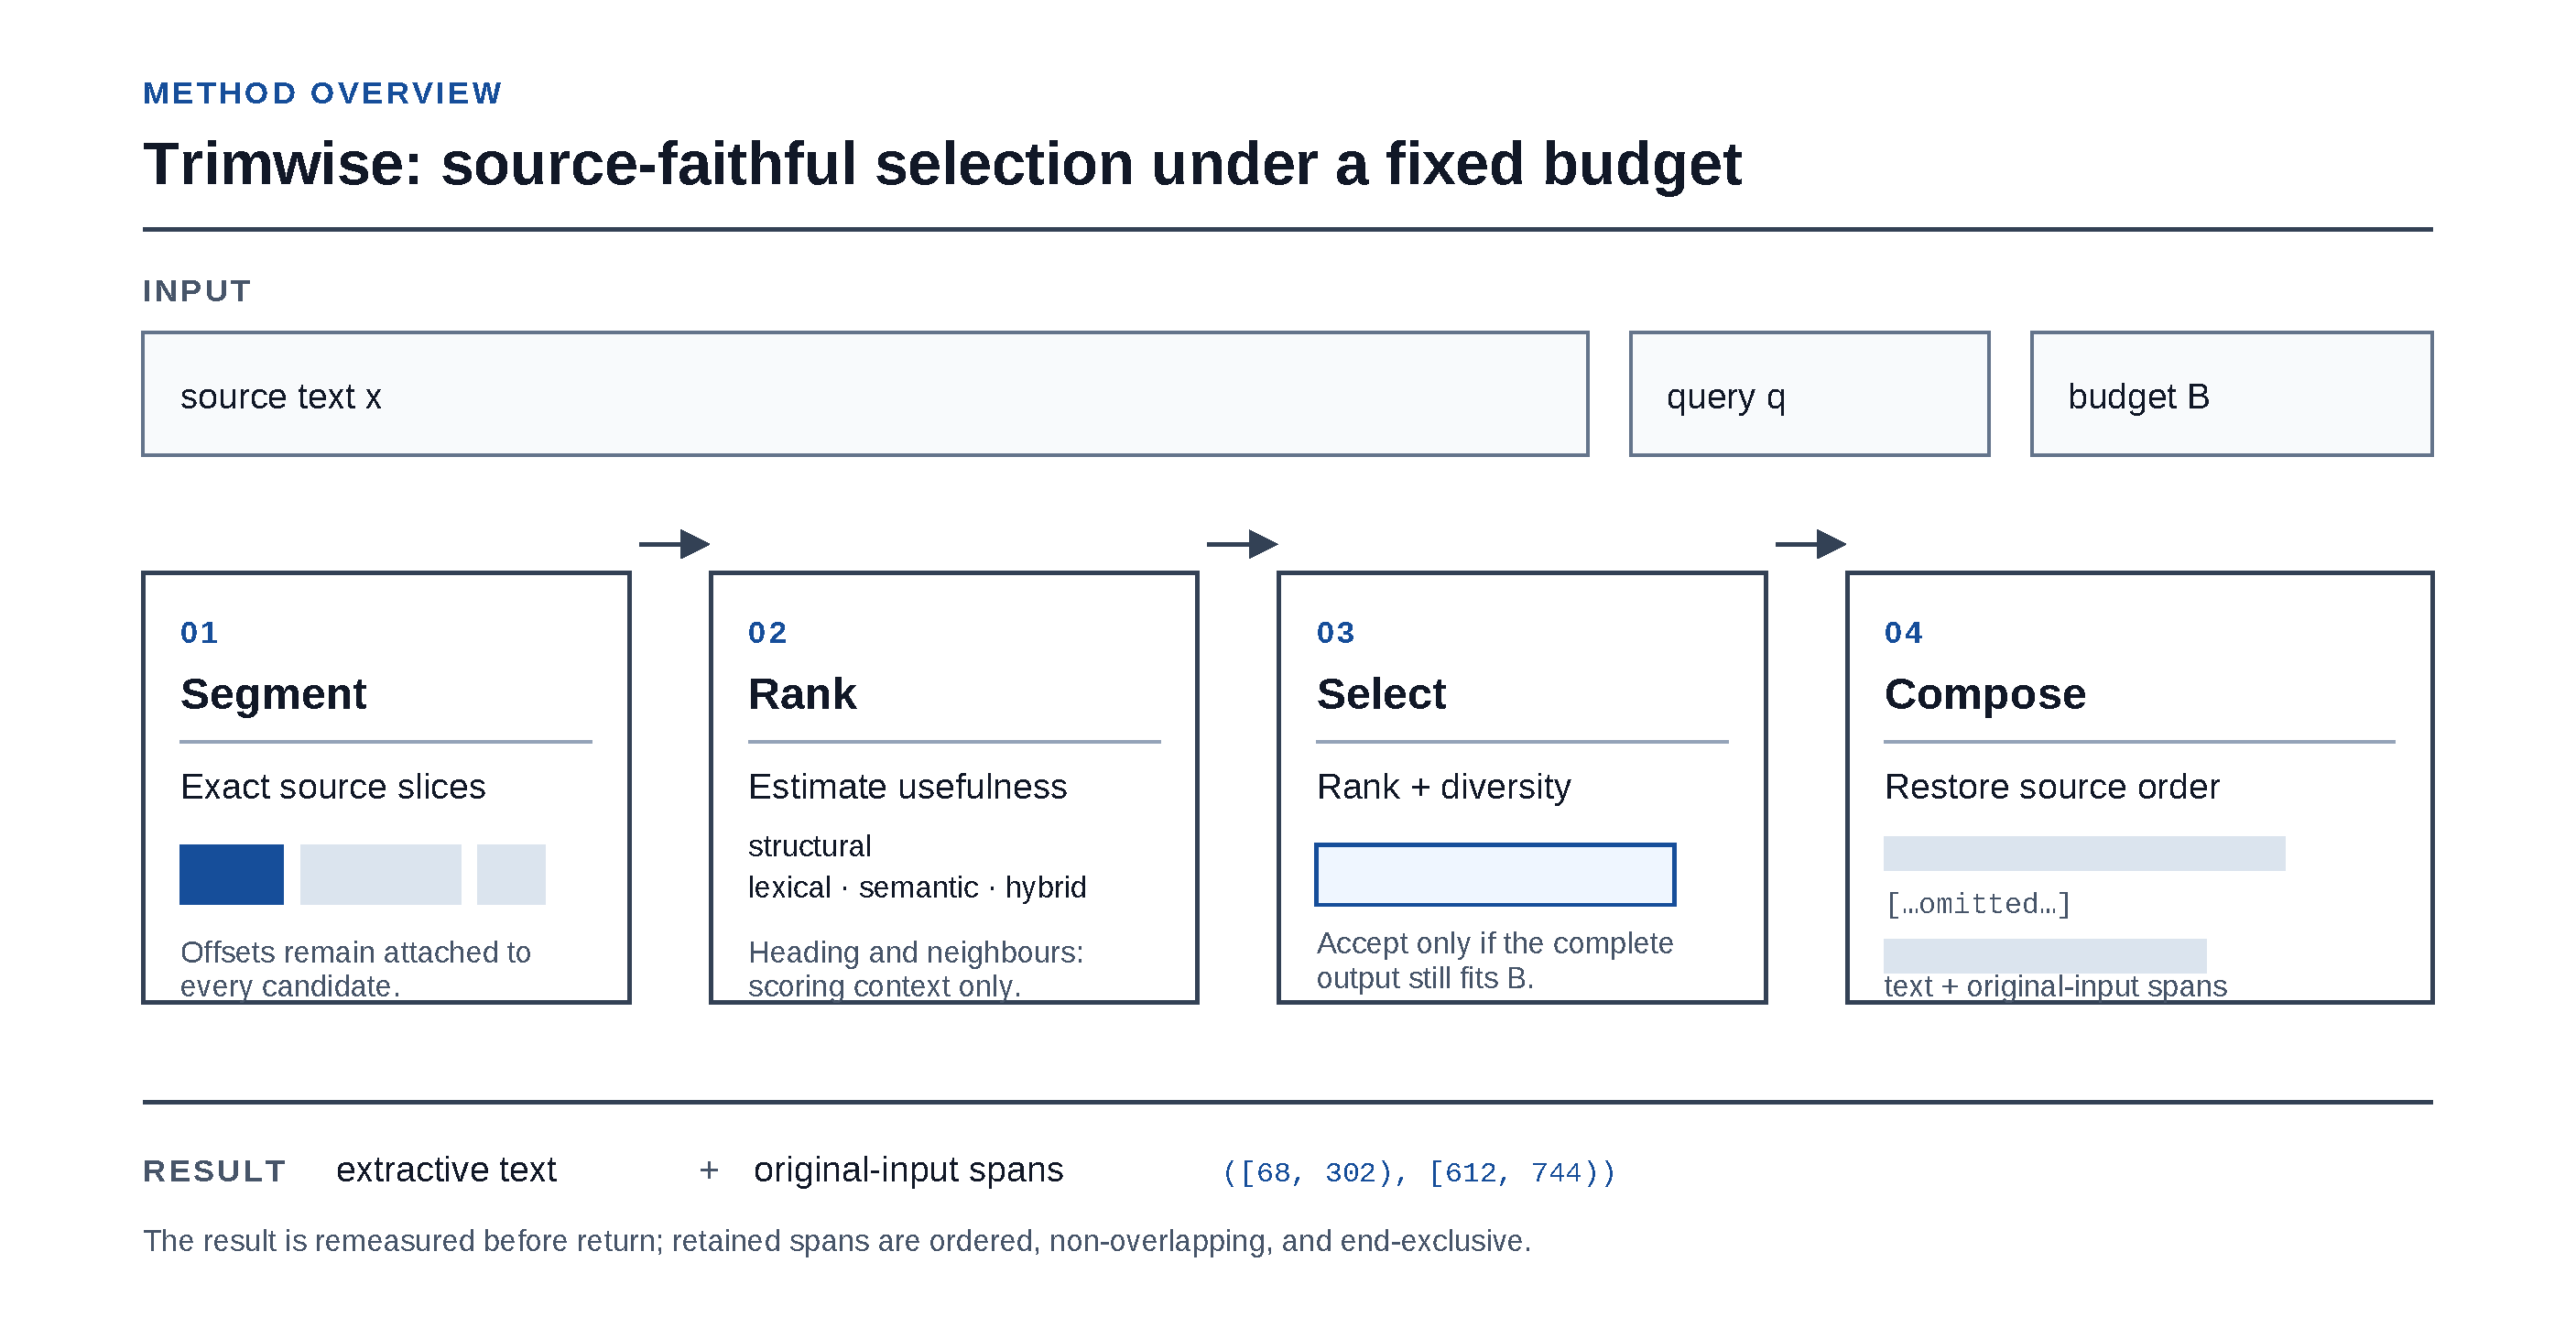
\includegraphics[width=\linewidth]{figures/trimwise-pipeline.pdf}}
\caption{Trimwise selection pipeline. Ranking may use structural, lexical,
semantic, or hybrid signals; selection and composition remain source-backed
and budget-aware.}
\end{figure}

Figure 1 shows the common path used by all strategies. Trimwise first
validates the request and measures the full source in the selected unit.
A source that already fits returns unchanged; an oversized source is
segmented into ordered candidates whose text is always an exact source
slice. The chosen strategy then assigns candidate relevance and supplies
the similarity representation used to discourage repeated evidence.
Structural selection uses document-level salience without a query;
lexical, semantic, and hybrid selection use a nonblank query. Ranking
context may include a candidate's nearby heading and neighbours, but
this enriched text is used only for scoring and is never emitted as a
replacement for the source candidate.

Selection is greedy and stateful. At each step, the method considers
relevance together with similarity to material already retained,
tentatively composes the proposed set in original source order, and
accepts the candidate only when the complete result still fits the
requested budget. The structural route additionally protects fitting
endpoint evidence and distributes provisional capacity across document
sections; the query-aware route bounds its evidence pool before the
greedy pass and can attach a selected passage's heading when it fits. If
no complete candidate can be accepted, the method uses an exact
fitting-source-prefix fallback. Finally, composition inserts only
affordable separators and omission markers, remeasures the text, and
returns the text together with its original-input spans. Thus all
strategies share the same provenance and budget boundary even though
they differ in how they estimate usefulness.

\subsection{Document Segmentation}\label{document-segmentation}

Segmentation defines the units that can be ranked, selected, and cited.
Trimwise begins from the original Python string rather than from
rendered Markdown. It parses oversized nonblank input with the
CommonMark rules of \texttt{markdown-it-py} and enables table support.
Parser line ranges are converted to character offsets using the input's
original line endings. For each candidate \(u_i\), the implementation
records its stable position, block kind, heading-derived section
metadata, and the half-open interval \([a_i,b_i)\) such that
\(u_i=D[a_i:b_i]\). The parser is used to find boundaries, not to
recreate text, so whitespace, indentation, link syntax, and code-fence
markers remain part of the exact source slice.

The parser identifies headings, paragraphs, tables, HTML blocks,
horizontal rules, indented code, and fenced code. Paragraphs inside
block quotes and ordered or unordered lists retain their container kind,
which lets later selection recognize list- and quote-backed units
without normalizing them. A closed leading YAML-style front-matter block
is retained as raw source. The implementation also closes a common
provenance gap in parser-driven systems: after it derives parser spans,
it inserts a raw candidate for every nonblank range that the parser did
not cover. Consequently, reference definitions or unusual syntax cannot
disappear merely because they were not emitted as a recognized block
token.

The resulting candidates are sorted by source position and made
non-overlapping. Identical parser ranges are deduplicated, favouring the
richer structural kind for known ties; a contained range is discarded,
and an unusual partial overlap is clipped at the preceding range's end.
Each heading starts a numbered section, and each later candidate keeps
the nearest preceding heading index. This metadata supports
section-aware structural selection and lets query-aware selection
include a passage's heading when doing so remains within budget. Empty
input has no candidates; whitespace- only input is represented as one
raw candidate so that the source model remains well-defined.

There is deliberately no global minimum or maximum candidate size
expressed in characters or tokens. Such thresholds would make structural
fidelity depend on a tokenizer before the method has selected any text.
They do, however, expose a pathological case: a long plain-text document
may be parsed as one paragraph and therefore offer only one rankable
candidate. In structural mode, when this is the entire candidate set,
Trimwise expands that paragraph into complete sentence or source-line
slices. Sentence boundaries cover \texttt{.}, \texttt{!}, \texttt{?},
the Unicode ellipsis, and common CJK terminal punctuation. If no such
boundary exists---for example, an unpunctuated single line---the
paragraph remains indivisible until the later exact-prefix fallback.
This expansion is currently specific to structural selection;
query-aware strategies operate on the original Markdown-derived
candidate set.

Segmentation therefore affects both quality and budget use. Coarser
units preserve more local context but may fail to fit even when a
smaller useful passage would; finer units offer more choice but can
detach a fact from its qualification or heading. Trimwise addresses that
trade-off through structure-preserving defaults and a narrow fallback,
rather than claiming that one granularity is optimal for every document
or task.

\subsection{Candidate Scoring}\label{candidate-scoring}

Every strategy produces a primary score for each candidate and then
converts it to the common relevance scale used by selection. Before
scoring, Trimwise constructs a local ranking passage for each candidate:
the candidate appears first, followed---when available---by its nearest
heading and immediate same-section neighbours. This context makes a
short source slice less ambiguous without changing the text eligible for
output. Ranking-only passages are normalized with Unicode NFKC, case
folding, whitespace collapse, and a leading space before Tiktoken
encoding. The normalized representation is never substituted for a
retained source fragment.

\subsubsection{Structural scoring}\label{structural-scoring}

Structural mode estimates representativeness when no query is available.
It adapts the centroid principle used in extractive summarization
\citep{radev-etal-2000-centroid} to the local ranking passages defined
above. Let \(V_i\) be the L2-normalized TF--IDF vector for candidate
\(u_i\), constructed from Tiktoken subword identifiers. For term \(t\)
in a candidate with \(L_i\) subwords, the unnormalized component is

\[
\operatorname{tfidf}_{i,t} = \frac{c(t,u_i)}{L_i}
\left(\log\frac{n+1}{\operatorname{df}(t)+1}+1\right),
\]

where \(n\) is the number of candidates and \(\operatorname{df}(t)\) is
the number of candidate passages containing (t). The document centroid
is the arithmetic mean of the normalized vectors,
\(C=n^{-1}\sum_i V_i\), and the primary structural score is

\[
p_i = \cos(V_i, C).
\]

This score favours candidates whose vocabulary is representative of the
supplied document. It is not a claim that such candidates are
universally important: a rare warning, exception, or final decision can
be essential precisely because it is unlike the document's average
language.

Trimwise min--max normalizes the primary-score vector within the
document. The final relevance used by the selector is a fixed blend

\[
r_i = 0.9\,\operatorname{minmax}(p_i) + 0.1\,g_i,
\]

where \(g_i\) is the mean of four binary signals: the candidate is a
heading or has a nearby heading, it contains a URL, it contains a number
or date-like value, or it contains a snake-case or camel-case
identifier. These lightweight indicators are intended to keep technical
and operationally specific evidence from being discarded solely because
it is lexically uncommon. They are not named-entity recognition, fact
verification, or a learned importance model.

When all primary scores are equal, min--max normalization yields zero
for every candidate; the small structural signal then supplies the only
score difference before the diversity-aware stage. Remaining ties
resolve toward the earlier source position. Thus structural mode is
deterministic for fixed text, configuration, and tokenization, but it
remains a queryless heuristic rather than a substitute for
task-conditioned evidence selection.

\subsubsection{Lexical relevance}\label{lexical-relevance}

Lexical mode uses Robertson BM25 \citep{robertson-zaragoza-2009-bm25} to
prioritize source passages that share discriminative terms with a
supplied query. A public lexical or hybrid call requires a nonblank
query; automatic mode resolves to lexical only when one is present. Both
the query and candidate ranking passages use the normalization described
above, then become Tiktoken subword identifier sequences. The
identifiers, rather than whitespace-delimited words, are the terms used
by the scorer. This is an implementation choice intended to retain
lexical evidence in technical identifiers and scripts for which
whitespace is not a reliable word boundary; it is not a claim that
Tiktoken tokenization improves BM25 in every language or domain.

For candidate \(u_i\), let \(f(t,u_i)\) be the frequency of query term
\(t\), \(L_i\) its subword length, \(\bar L\) the mean candidate length,
and \(\operatorname{df}(t)\) the number of candidates containing (t).
Trimwise computes

\[
p_i = \sum_{t \in \operatorname{unique}(q)}
\log\!\left(1 + \frac{n-\operatorname{df}(t)+0.5}
{\operatorname{df}(t)+0.5}\right)
\frac{f(t,u_i)(k_1+1)}
{f(t,u_i)+k_1\left(1-b+b\frac{L_i}{\bar L}\right)},
\]

with \(k_1=1.5\) and \(b=0.75\). Query terms are deduplicated before the
sum, so repeating a word in the question does not raise its
contribution; repeated occurrences inside a candidate still have the
usual BM25 saturating effect. As in structural mode, the primary scores
are min--max normalized within the source and combined with the same
10\% lightweight structural and fact-like signal before diversity-aware
selection.

BM25 rewards literal overlap, not paraphrase or entailment. It is
therefore appropriate when the query names a function, identifier, error
string, URL, date, or other exact source wording. It can miss a relevant
passage expressed with different vocabulary, and a lexical match can
still be a false lead. Semantic and hybrid scoring address the first
limitation through embeddings; neither changes the source-fidelity or
budget contracts described above.

\subsubsection{Semantic relevance}\label{semantic-relevance}

Semantic mode ranks a query against the same contextual candidate
passages used by the lexical scorer. It represents the query and each
passage as vectors and ranks them by cosine similarity, following the
sentence-embedding retrieval pattern
\citep{reimers-gurevych-2019-sentence}. Embedding quality remains a
property of the chosen model and domain.

For a query vector \(v_q\) and candidate-passage vector \(v_i\),
Trimwise validates that one query vector and exactly one passage vector
per candidate were returned, converts all vectors to a single
\texttt{float32} matrix, checks that they are finite and share one
nonzero dimension, and L2-normalizes each row. The primary semantic
score is then

\[
p_i = \hat{v}_q^\top \hat{v}_i,
\]

where hats denote normalized vectors. A zero vector remains zero after
normalization and therefore contributes zero cosine similarity. As with
the preceding strategies, Trimwise min--max normalizes the primary
scores within the source and combines them with the fixed lightweight
signal before selection. The passage vectors also provide the dense
similarity representation used later by the diversity objective.

Embeddings may be supplied by the application or generated through an
optional FastEmbed backend. The application-owned path leaves model
choice, batching, caching, authentication, and concurrency to the
application; Trimwise validates the returned vectors before scoring. The
execution boundary is an implementation detail and does not alter the
selection algorithm.

For the managed path, the default model identifier is
\url{sentence-transformers/paraphrase-multilingual-MiniLM-L12-v2}
\citep{sentence-transformers-paraphrase-multilingual-minilm-l12-v2}. Its
model card describes a 384-dimensional sentence-and-paragraph embedding
model covering 50 languages. The identifier is configurable. A
reproducible managed-backend experiment records the FastEmbed version,
provider options, and model revision or artifact hash observed at run
time; an application-supplied path records the corresponding model or
service details.

Cosine similarity captures proximity in an embedding space, not factual
correctness, authority, recency, negation, or joint answer sufficiency.
The evaluation therefore measures semantic ranking on the intended task.

\subsubsection{Hybrid relevance}\label{hybrid-relevance}

Hybrid mode retains both query signals: BM25 supplies the lexical
primary-score vector \(p_i^{\mathrm{lex}}\), and embeddings supply the
semantic vector \(p_i^{\mathrm{sem}}\). When every value is finite and
neither vector is constant, Trimwise independently min--max normalizes
the two vectors and uses the fixed equal blend

\[
p_i = 0.5\,\operatorname{minmax}(p_i^{\mathrm{lex}})
    + 0.5\,\operatorname{minmax}(p_i^{\mathrm{sem}}).
\]

Convex score combination and rank-based alternatives are established
forms of hybrid retrieval fusion
\citep{bruch-gai-ingber-2023-hybrid-fusion}. The equal weight above is a
Trimwise implementation choice: it is neither learned during selection
nor exposed as a public tuning parameter. It should not be read as an
assertion that 0.5 is optimal for all source collections, embedding
models, or downstream tasks. The fused primary vector is subsequently
passed through the same 90/10 relevance and lightweight-signal blend
used by the other strategies.

If either raw score vector is non-finite or constant, min--max magnitude
is not informative. In that case Trimwise uses one-indexed Reciprocal
Rank Fusion (RRF) \citep{cormack-clarke-buettcher-2009-rrf} with
\(k=60\):

\[
p_i = \frac{1}{60+\operatorname{rank}_{\mathrm{lex}}(i)}
    + \frac{1}{60+\operatorname{rank}_{\mathrm{sem}}(i)}.
\]

Ranks are sorted by descending raw score and break ties toward earlier
source positions. RRF is a defensive fallback rather than the normal
hybrid path; it preserves ordering information when the two score scales
cannot be compared safely. In both paths, hybrid selection uses the
semantic passage vectors---not the fused scalar scores---to measure
redundancy during the later diversity pass.

Hybrid mode consequently inherits the embedding requirements, runtime
cost, and embedding-model limitations of semantic mode, as well as the
lexical behaviour of BM25. It can retain evidence that is strong by
either signal, but it cannot guarantee that the two signals are
complementary or that their combination improves a particular task.
Those are empirical questions addressed only by the evaluation.

\subsection{Diversity-Aware Selection}\label{diversity-aware-selection}

Ranking candidates independently can spend most of a small budget on
passages that repeat one claim. Trimwise therefore applies a greedy
maximal marginal relevance (MMR) rule, adapting the
relevance--redundancy trade-off used for diversity-aware reranking
\citep{goldstein-carbonell-1998-mmr}. Given already selected candidates
\(S\), it scores each remaining candidate \(u_i\) as

\[
\operatorname{MMR}(u_i) = \lambda r_i
  - (1-\lambda)\max_{u_j \in S}\operatorname{sim}(u_i,u_j),
\]

where \(r_i\) is the final relevance from §4.4 and the maximum
similarity is zero before the first selection. The public configuration
parameter \(\lambda\in[0,1]\) defaults to \(0.7\), giving relevance a
70\% weight and redundancy a 30\% penalty. This setting is a library
default, not a learned optimum or a claim that the same trade-off fits
every task.

The similarity representation follows the ranking path. Structural and
lexical strategies use cosine similarity between their sparse TF--IDF
vectors; semantic and hybrid strategies use nonnegative cosine
similarity between normalized passage embeddings. After each accepted
main candidate, Trimwise updates every remaining candidate's largest
observed similarity instead of recomputing similarities to all prior
selections. For dense embeddings this update is vectorized; for sparse
representations it is an exact pairwise pass. Maintaining this state
costs \(O(kn)\) similarity updates for \(k\) accepted candidates among
\(n\) candidates, excluding the separate cost of constructing
representations and repeatedly checking whether a proposed excerpt fits
its budget.

The surrounding selection policy differs by strategy. Structural mode
first attempts to preserve fitting endpoint candidates, allocates
provisional capacity across source sections, and then fills the
remaining space by the live MMR score. Query-aware modes exclude
standalone headings from the initial evidence pool, limit that pool
using the primary-score distribution, and then use the same MMR pass; an
accepted passage may bring its nearest heading if the combined
composition fits. In all cases, equal MMR scores break toward the
earlier candidate position, making selection deterministic for fixed
input, configuration, measurement, and embedding vectors.

MMR measures similarity of representations, not independent facts. A
paraphrase can look diverse, two distinct facts about the same entity
can look redundant, and a candidate that would complete an answer can
still be rejected if it scores poorly or fails the remaining budget. The
method therefore reduces representational repetition; it does not
guarantee factual diversity, complete coverage, or globally optimal
subset selection.

\subsection{Budget-Constrained
Packing}\label{budget-constrained-packing}

Trimwise enforces a budget on the composed excerpt, not on a list of
independently sized candidates. The measurement rule is selected by the
caller: characters use Python string length, words use
whitespace-separated parts, and token budgets use the configured
Tiktoken encoding (default \texttt{o200k\_base}) or a caller-provided
counter. For every tentative selection, the method sorts the retained
candidates by source position, constructs the entire prospective output,
and measures that string. A candidate or query-aware
candidate-plus-heading bundle is accepted only when the resulting count
is at most the requested budget. Exact boundary cases therefore fit;
there is no separate rounding allowance.

Composition first includes retained source fragments and the whitespace
already present between adjacent fragments when the omitted source gap
contains only whitespace. If an omitted gap contains non-whitespace
source content, the initial composition uses at most one blank line as a
minimal separator. The candidate bundle is rejected immediately if this
source-and-separator form exceeds the budget. Only after source content
fits does Trimwise attempt to replace leading, internal, and trailing
gaps with the configured omission marker. Each replacement is tried in
source order and kept only if remeasuring the full result still
satisfies the bound. Consequently, an omission marker never displaces
retained evidence, and its absence does not imply that the selected
source fragments were adjacent.

This procedure makes candidate size context-dependent: adding a passage
can change the separator, heading attachment, and affordable marker
decisions around passages already selected. It also explains why the
selector may leave capacity unused. Query-aware selection can exhaust
its bounded evidence pool; no remaining complete candidate may fit; or
only an optional marker may be too large. The method does not add weak
evidence merely to make the output count approach the limit.

Normal selection never splits an accepted structural candidate. If no
complete candidate can fit, Trimwise instead invokes a fallback on the
highest-relevance candidate, breaking ties toward the earlier source
position. It first seeks the longest fitting prefix at paragraph
boundaries, then at complete sentence or line boundaries, and finally
uses the longest exact prefix measurable under the requested rule.
Fenced code receives a narrower special case: when its opening and
closing fences fit together, the fallback keeps a balanced fence and the
longest fitting body prefix at a line boundary; otherwise it follows the
ordinary exact-prefix path. The fallback preserves source text, but
under a very small budget it can necessarily cut through a
natural-language unit.

The zero-budget case returns an empty excerpt. All other returned paths
are measured after their final composition, including any fallback
markers, so the independently auditable invariant remains
\(\mu(T)\leq B\). The next subsection specifies how the source-backed
portions of that composed text are reconstructed and exposed to callers.

\subsection{Source-Order
Reconstruction}\label{source-order-reconstruction}

Relevance order answers which candidates were selected; it is not a
readable or citable presentation order. A highly relevant conclusion may
rank above its prerequisite, and two selected passages may be far apart
in the source. Before composing every tentative selection, Trimwise
sorts candidate indexes by their original source position. It then emits
the exact source slices in that order and applies only the separator and
omission-marker rules described in §4.6. Thus a later selected passage
cannot appear before an earlier selected passage merely because it
received a higher score.

The public result exposes this relationship through
\texttt{SourceSpan(start,\ end)} values. Offsets refer to the original
Python string passed to \texttt{trim()} or \texttt{atrim()}:
\texttt{start} is inclusive and \texttt{end} is exclusive, so
\texttt{source{[}span.start:span.end{]}} recovers the corresponding
source-backed text exactly. The spans are ordered and non-overlapping.
They are also maximal rather than one-to-one with internal candidates:
selected candidates separated only by copied source whitespace are
merged into one span, as are adjacent candidates. A gap containing
omitted non-whitespace source content starts a new span.

This rule distinguishes provenance from display formatting. If the
result joins non-adjacent spans, the source slices identify precisely
what was retained, while a minimal newline separator or an omission
marker explains the display boundary when it fits. Generated separators
and omission markers have no source span. A caller can therefore
reconstruct the retained source material by reading the spans in order
and can reconstruct the displayed excerpt by inserting only the
non-source layout elements that Trimwise returned. In the special
balanced-fence fallback, for example, the opening portion and closing
fence are represented by two source spans even though they appear
together in the output.

The unchanged-input path is intentionally simple: a nonempty input that
already fits returns one span from zero to the input length, and an
empty result returns no spans. These values are sufficient for a prompt
assembler to intersect retained character ranges with its own
repository-relative path and line map. Trimwise does not return document
identifiers, file paths, permissions, line/column ranges, or source
ownership metadata; those belong to the application that supplied the
string.

Source order and recoverable offsets improve inspection and citation,
but they do not restore omitted context. A span can contain an exact
conclusion while its definition, qualification, or contradiction lies
outside the selected ranges. Reconstruction is therefore a provenance
guarantee, not a guarantee of semantic completeness or answer
correctness.

\subsection{Complexity and
Implementation}\label{complexity-and-implementation}

Let \(n\) be the number of segmented candidates, \(r\) the total number
of Tiktoken subword IDs in their contextual ranking passages, \(d\) the
embedding dimension when semantic scoring is used, and \(k\) the number
of accepted main candidates. Let \(C(B)\) denote the cost of composing
and measuring one tentative output at the requested budget scale \(B\).
This notation separates work under Trimwise's control from embedding
inference and from a caller-provided token counter, whose cost is
external to the library.

Markdown parsing, source-offset construction, and candidate bookkeeping
are linear in the input size under the parser's normal execution path.
Building contextual ranking passages and tokenizing them is linear in
\(r\). Structural scoring constructs sparse TF--IDF vectors, their
centroid, and candidate--centroid similarities in time proportional to
the nonzero token representation; its working memory is likewise sparse
in that representation. Lexical scoring uses the same tokenized passages
and, after term-frequency construction, evaluates the unique query terms
against each candidate. It requires no embedding model.

Semantic scoring has two parts. Trimwise's vector validation,
normalization, and query--passage dot products take \(O(nd)\) time and
\(O(nd)\) memory. The embedding call itself is deliberately not assigned
a fixed asymptotic or latency here: it depends on the caller's model or
service, its batching, provider, hardware, cache state, and input
lengths. Hybrid scoring performs both lexical and semantic work, then
adds an \(O(n)\) score-fusion pass. These distinctions matter
operationally: the structural and lexical paths are local sparse
computations, whereas semantic and hybrid paths are usually dominated by
embedding inference.

The exact MMR update maintains a maximum similarity for every remaining
candidate after each accepted candidate. With sparse representations,
this takes \(O(kn\bar{s})\) similarity work, where \(\bar{s}\) captures
the average sparse-vector comparison cost; with dense embeddings,
vectorized updates take \(O(knd)\). Greedy choice itself scans the
remaining candidates. When the current highest-MMR proposal does not
fit, the implementation orders the remaining candidates to search for
another fitting one; this retry path can add sorting overhead in
unfavorable packing cases. It is kept exact rather than replaced with an
approximate-neighbour index because the intended workloads are bounded
prompt excerpts, not a corpus-scale retrieval service.

Budget enforcement also has a visible cost. Each candidate or
candidate-plus-heading proposal is recomposed and remeasured, so
selection performs \(O(n)\) trial compositions in the ordinary pass,
with a constant number of additional attempts for a heading bundle.
There is no cached knapsack approximation: output order, separators,
omission markers, and tokenizer behaviour can change the cost of a
candidate in context. The resulting time includes approximately
\(O(nC(B))\) composition and measurement work, plus the retry-order
overhead above. A custom counter can make \(C(B)\) substantially more
expensive; this is the price of preserving the caller's measurement
contract.

Trimwise is implemented in Python and this manuscript describes package
version 0.2.0. Its core dependencies are \texttt{markdown-it-py} for
source-aware parsing, NumPy for vector operations, and Tiktoken for
default token measurement and lexical terms. Semantic inference is
optional through the \texttt{fastembed} or \texttt{fastembed-gpu}
extras, while an application may instead supply embeddings from its own
model or service. The experiment record identifies the selected backend
and its relevant model configuration.

\section{Experimental Setup}\label{experimental-setup}

\subsection{Research Questions}\label{research-questions}

The primary evaluation concerns query-aware selection from one
already-chosen source. Every method within that comparison receives the
same case query during compression; depending on the task, that query is
a question, instruction, procedure, or structured-data request.
Source-only methods are reported in a separate diagnostic and are not
pooled into the query-aware aggregate. The research questions below
define the main evaluation and its reporting boundaries.

\textbf{RQ1 --- Evidence preservation and task utility.} Under a shared
query and token budget, how often does each method retain the required
source evidence and satisfy the case-level task conditions? The primary
source-level outcome is normalized contiguous required-span containment:
all required evidence must survive as complete normalized passages,
prohibited content must be absent, and the output must respect the
requested budget. Where a case defines an answerable downstream task,
answer outcomes are reported separately rather than substituted for
source-evidence preservation.

\textbf{RQ2 --- Position robustness.} Does evidence-preservation
performance change when required evidence occurs at the beginning,
middle, end, or multiple locations in the source? The
position-controlled set has 40 cases in each stratum. Results report
both stratum-level values and aggregates over this balanced set so that
a front-loaded corpus cannot hide position-specific failures.

\textbf{RQ3 --- Budget behaviour.} How do methods trade source-evidence
preservation against output size across 128, 256, 512, and 1,024 token
ceilings? This question includes budget violations, actual output-token
ratio, and token savings. High budget utilization alone is not
considered evidence of quality: a method can fill a budget with
irrelevant or unsafe text, while an evidence-bounded query-aware method
can correctly return less than the available ceiling.

\textbf{RQ4 --- Downstream answer transfer.} When the compressed context
is supplied to a fixed answering model, how does answer success compare
among compressed methods and against the untrimmed-context reference?
This question is evaluated only on cases with answerable ground truth
and reported by evaluator model. It does not treat the full-context
reference as a compression method or assume that better source-span
coverage must always produce a better generated answer.

\textbf{RQ5 --- Efficiency and reliability.} What trimming latency,
output-token reduction, failure rate, budget-compliance rate, peak GPU
memory, and thermal intervention does each method exhibit under a common
runtime protocol? Compression time and thermal waiting are recorded
separately, since a cooldown policy protects the hardware but is not
algorithmic work. Comparisons are scoped to the recorded hardware,
software versions, model cache state, and method-specific dependencies.

The present protocol compares complete methods, not independent switches
for segmentation, relevance, diversity, and reconstruction. It therefore
cannot make a causal component-ablation claim. Such a claim requires a
separate frozen ablation study in which each component is disabled or
replaced while all other choices remain fixed.

\subsection{Tasks and Datasets}\label{tasks-and-datasets}

The primary dataset is a separate, position-controlled set of 160 cases
derived from a frozen 250-case source corpus containing 150 documents.
Each case supplies one context string, a task query, source-backed
required evidence spans, and, where applicable, a reference answer,
ordered steps, and prohibited phrases. The source corpus was frozen
before method execution, uses seed 20260718, and has SHA-256 digest
\texttt{7b752ea79f19369fa151aa27f8bcfb33abdc48d9a9da609b655640e931c7d428}.
The evaluation set is therefore a fixed derived artifact, rather than a
sample selected after inspecting compressor results.

The original 250-case corpus remains unchanged; the separate 160-case
evaluation contains 135 natural cases and 25 controlled relocations.

The cases cover six task tracks: 46 evidence-question-answering cases,
30 real-source evidence cases, 26 instruction-survival cases, 21
structured-data cases, 20 procedure-survival cases, and 17 adversarial
cases. Their sources mix controlled synthetic incidents, policies,
procedures, structured records, and adversarial documents with public
permissively licensed code, documentation, research, data,
security-policy, and specification excerpts. The source manifest records
a URL, revision where available, and license for each public document;
controlled synthetic documents are marked CC0-1.0. This is a task suite
for source-evidence selection, not a benchmark of broad world knowledge
or document summarization.

Evidence position is an explicit experimental factor. The set contains
exactly 40 cases with all required evidence near the beginning of the
context, 40 in the middle, 40 at the end, and 40 with required evidence
in multiple locations. Of these rows, 135 preserve their natural source
placement; 25 are controlled end-position variants. For each variant,
one required span that occurred exactly once in an unused source case was
moved unchanged to the end of the same context; the original source case
was excluded from the 160-case set. The
construction script verifies the new offsets, exact required text,
unique provenance, distinct variant source documents, and the
40/40/40/40 balance. The accompanying review manifest records every
variant and its parent case.

\begin{figure}
\centering
\pandocbounded{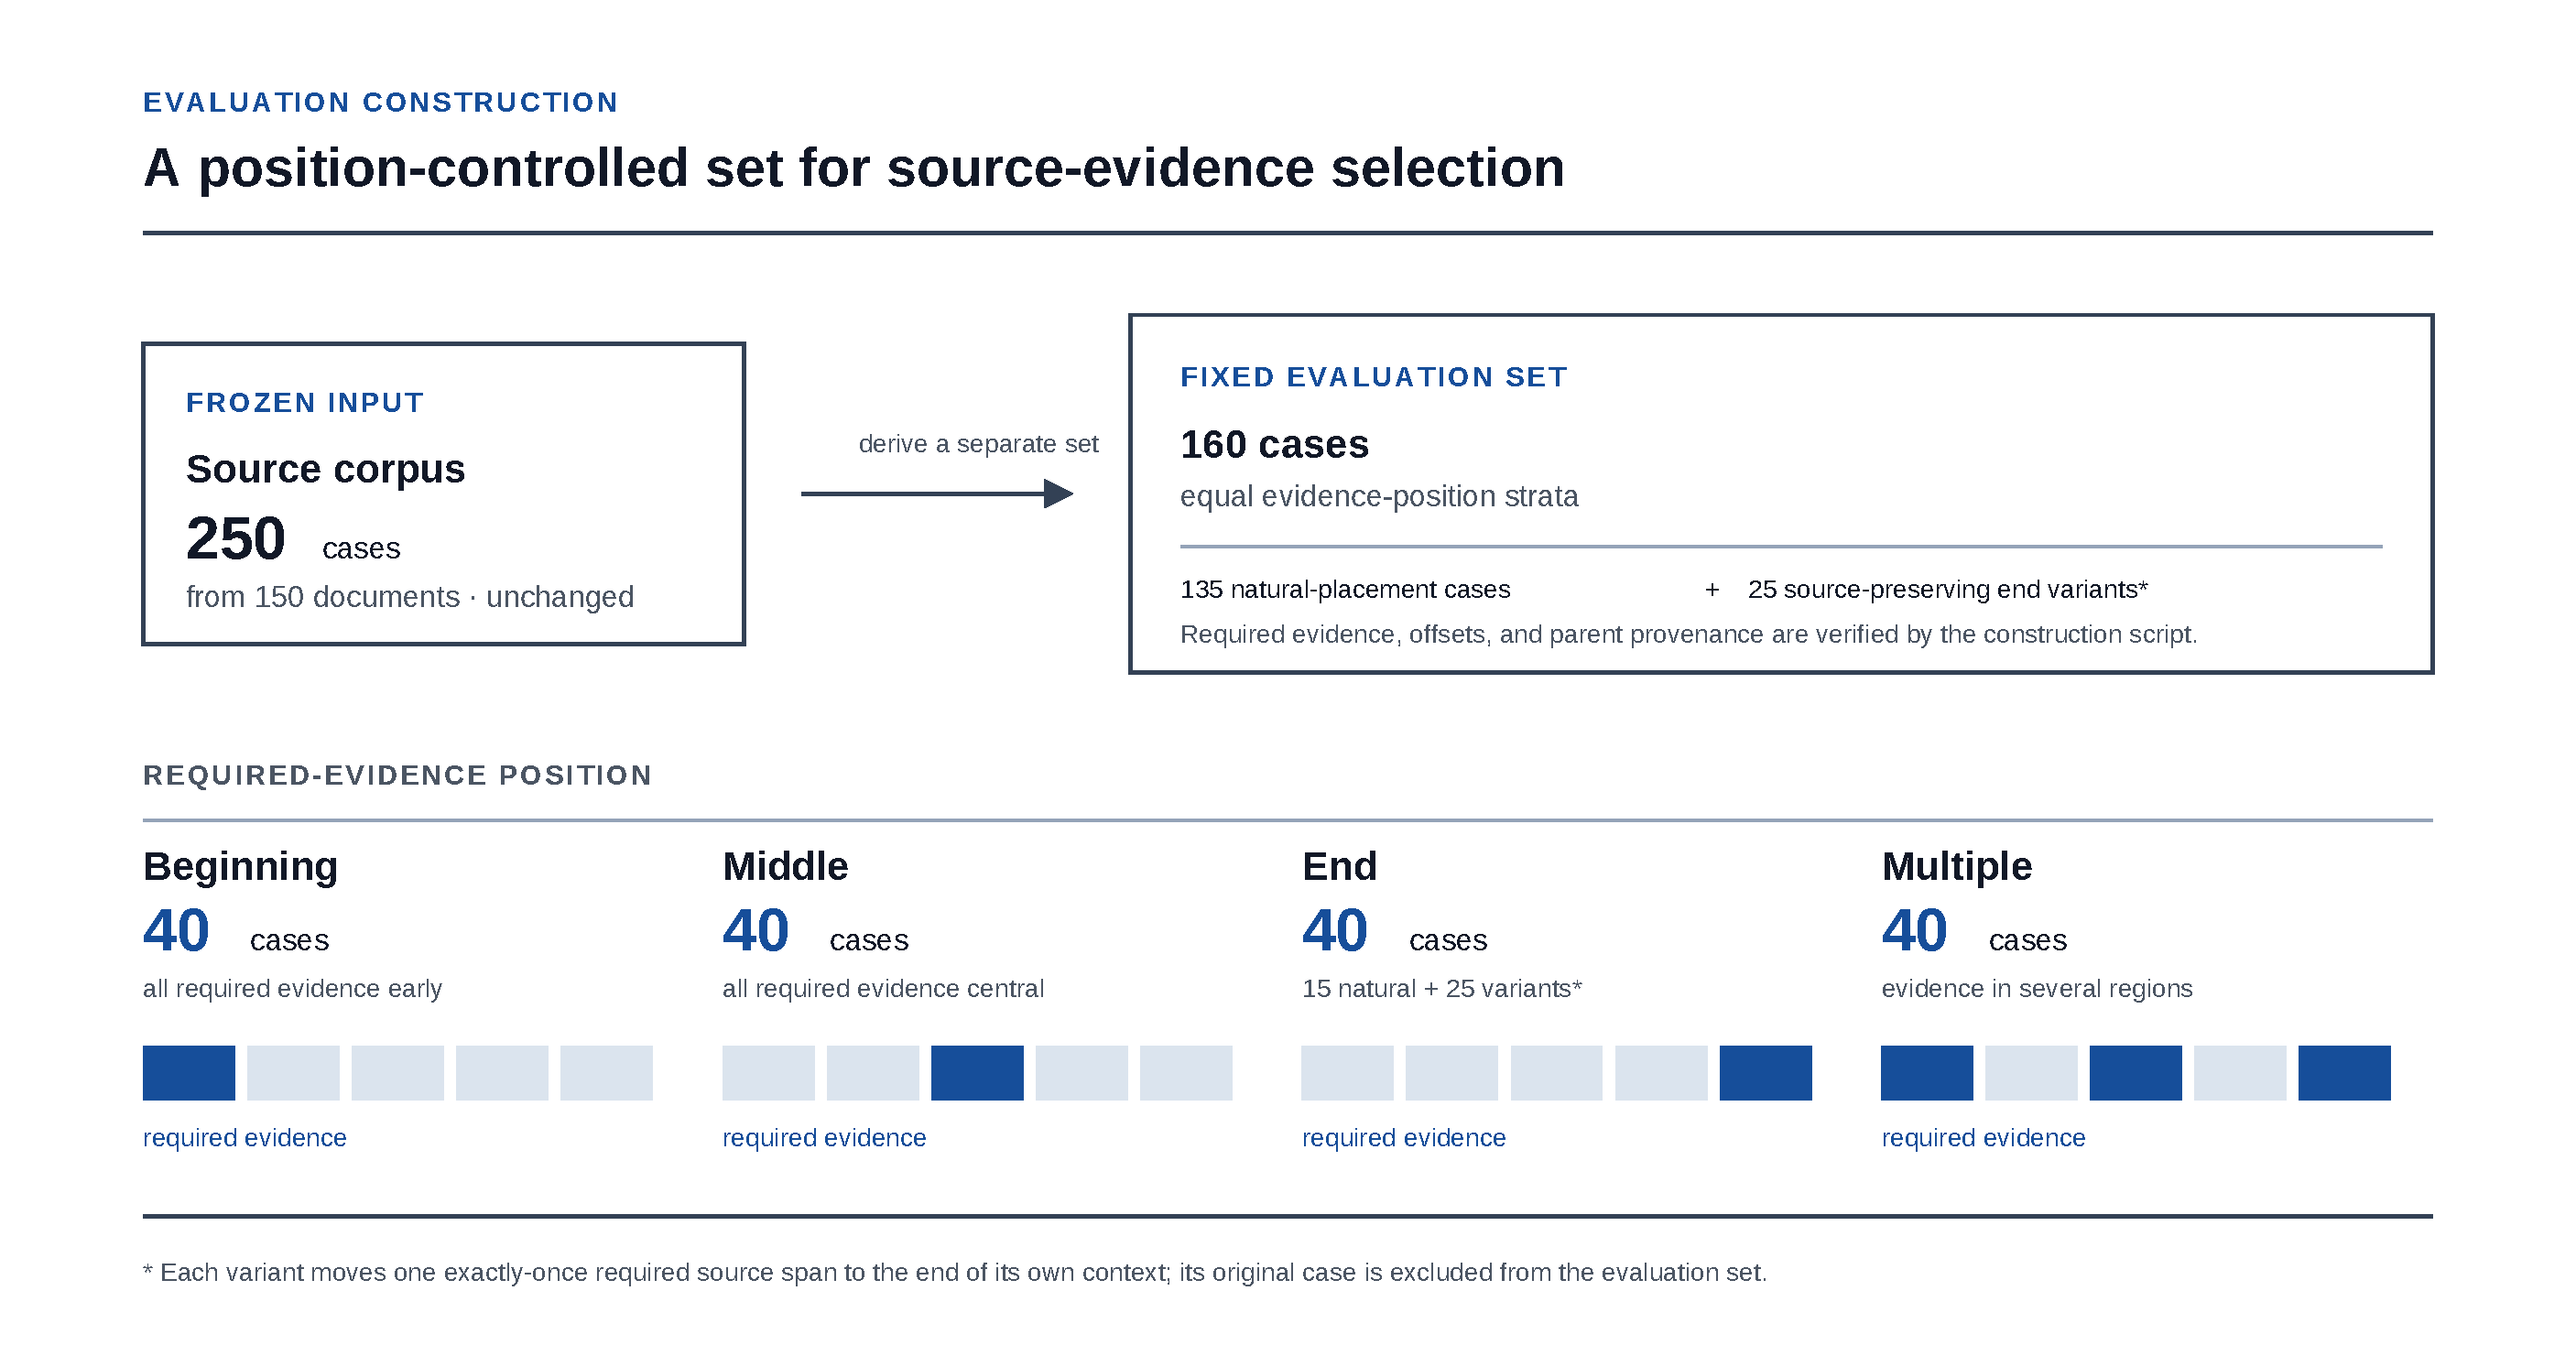
\includegraphics[width=\linewidth]{figures/position-controlled-160.pdf}}
\caption{Position-controlled construction of the 160-case evaluation. The
original 250-case source corpus remains unchanged; the separate evaluation set
has 135 natural cases and 25 controlled relocations. It has 40 cases in every
evidence-position stratum, including 25 provenance-linked, source-preserving
end relocations.}
\end{figure}

This construction addresses a concrete threat to positional benchmarks:
a prefix method can appear strong when most evidence happens to be
early. It does not create a fully natural distribution of end-position
evidence. In particular, relocation changes local discourse context
around a required span and should be interpreted as a controlled
diagnostic, not as a claim that all long documents end with an isolated
answer. We consequently report results by position as well as aggregates
over the position-balanced set. We also re-aggregate the saved rows after
excluding all 25 relocations. This 135-case natural-only sensitivity
analysis contains 40 beginning, 40 middle, 15 end, and 40 multiple-evidence
cases; it is intentionally not position-balanced. No compressor or evaluator
is run again for this analysis. A second saved-output sensitivity excludes all
10 	exttt{real-trimwise-*} cases drawn from four Trimwise documents. It tests
whether the observed comparison is dependent on the author's own source domain;
the 150 remaining cases are not rebalanced.

Contexts range from 1,423 to 100,897 Python characters, with a median of
9,362 characters. There are 120 cases with one required span, 6 with
two, 28 with three, and 6 with four. The tracks are not equally sized;
aggregate primary-metric rates weight each of the four position strata
equally because the set is balanced, while the separately reported macro
rate weights task tracks equally. Track-level results remain necessary
to expose task-specific failure modes. The corpus has no
development/test split because it is a single fixed comparative
evaluation suite. Compressor configurations and the original v1.1
evaluation were fixed before the final compression run; the v1.2 metric
protocol was separately frozen before rescoring the saved outputs. No
method parameters were tuned on a held-out subset of these 160 cases.

Public-source examples and the source code of Trimwise itself may have
appeared in the training data of the downstream language models. The
controlled synthetic documents avoid that particular public web exposure
but are not a substitute for a formal contamination audit. The
evidence-retention metric is based on supplied source spans and is not
affected by a model's prior knowledge; generated answer outcomes, by
contrast, can be. We therefore interpret answer results as a downstream
diagnostic alongside source-evidence outcomes, not as proof that a model
relied exclusively on the retained context.

The compression run has two access conditions. The primary query-aware
condition gives every included method the context and its case query. A
separate source-only condition gives its methods only the context; its
query is shown later to the answering model. The two conditions answer
different questions and are never pooled, ranked, or used to claim that
one access condition is better than the other.

\subsection{Baselines}\label{baselines}

The main comparison is deliberately limited to methods that accept a
case query and were run through the same compression runner on the same
source strings, budgets, and post-hoc token counter. It contains
Trimwise Lexical, Trimwise Hybrid, an LLMLingua GPT-2 token-pruning
adapter, a LongLLMLingua GPT-2 single-context adapter, and a RECOMP NQ
extractive sentence adapter. Trimwise Lexical uses its built-in BM25
relevance path; Trimwise Hybrid adds the managed embedding backend and
hybrid fusion described in Section 4. Both LLMLingua adapters are invoked
through \texttt{llmlingua==0.2.2} with \texttt{openai-community/gpt2} on
CUDA. The token-pruning adapter enables token-level filtering and
preserves original order. The single-context adapter passes the complete
source as one context string, enables context- and token-level filtering,
uses \texttt{dynamic\_context\_compression\_ratio=0.3}, and permits its
configured ranked context ordering.

The RECOMP NQ extractive sentence adapter needs a more precise description
than its family name alone conveys. The benchmark loads
\texttt{fangyuan/nq\_extractive\_compressor} through Transformers,
mean-pools its query and sentence representations, ranks source
sentences by dot product, and greedily packs whole sentences under the
common token counter. It is an extractive benchmark adapter built around
the released model identifier, not a claim that every preprocessing and
decoding detail of the published RECOMP system has been reproduced. This
distinction is material when interpreting either quality or latency.

For the source-only diagnostic, the runner separately includes
first-\emph{N} prefix truncation, head--tail truncation, Trimwise
Structural, LLMLingua without a query, and LLMLingua-2. These methods
receive an empty compression query. They are reported on their own
access-condition page and are not placed in a headline query-aware
ranking. Selective Context was explored during benchmark development but
is excluded from the frozen run because its runtime made the planned
comparison impractical; it must not appear as an unrun baseline in
tables or narrative.

Every method receives a requested target of 128, 256, 512, or 1,024
tokens. The runner treats the method's own output as its output, then
scores it with the common \texttt{o200k\_base} counter used by Trimwise.
A target passed to a baseline is therefore not assumed to be a guarantee
under that counter; measured budget violations are reported. This avoids
silently treating different internal tokenizers as interchangeable,
while retaining the native configuration that each method requires.

The saved compression rows were generated before the 0.2.0
provenance-span release. A direct implementation comparison confirms
that the 0.2.0 change adds span propagation and public result metadata
without changing segmentation, ranking, or emitted-text selection. The
observed source-evidence and answer scores therefore describe the same
selection path now installed by the benchmark environment, while the
historical raw rows themselves do not contain span arrays.

\subsection{Budget Regimes}\label{budget-regimes}

Each compressor is evaluated at absolute ceilings of 128, 256, 512, and
1,024 tokens under the shared \texttt{o200k\_base} counter. These levels
represent, respectively, a very constrained excerpt, a constrained
excerpt, a moderate excerpt, and a light-trimming ceiling. Absolute
limits make the selection problem comparable across documents whose
original lengths differ substantially; retained percentages are reported
only as descriptive output ratios. The same four limits apply to every
method in each access condition and to the compressed contexts passed to
the downstream QA runner.

The source context is the only text subject to compression. The task
query, protected instruction prefix, and protected suffix remain outside
the compressible payload and are assembled after compression for
downstream QA. This reflects the intended prompt-assembly use case:
application instructions are required context, while an optional source
excerpt must fit a separately allocated budget. It also avoids awarding
a compressor for deleting the task it is expected to support.

\subsection{Downstream Models and Inference
Protocol}\label{downstream-models-and-inference-protocol}

Downstream answer transfer is evaluated with three Responses API model
identifiers: \texttt{gpt-5.4-nano-2026-03-17},
\texttt{gpt-5.4-mini-2026-03-17}, and \texttt{gpt-5.6-luna}. The saved
runs were completed on 27 July 2026 (Asia/Kolkata). Each model receives
the same protected prompt template: an instruction to answer only from
the supplied context, the full or compressed context, the case-specific
protected suffix containing the task query, and a final request for only
a concise answer. The API call sets \texttt{max\_output\_tokens=128},
\texttt{reasoning.effort="none"}, \texttt{text.verbosity="low"}, and
\texttt{store=false}; requests have a 120-second timeout and a shared
maximum of 16 concurrent calls.

For every case and evaluator, the protocol includes one uncompressed
full-context reference and one answer for every successful compressor
output at every budget. This yields 6,560 saved rows per evaluator: 160
full-context rows plus \(160 \times 10 \times 4\) compressed-context
rows. The answer analysis is restricted to the adversarial, evidence-QA,
and real-source tracks, which have answer ground truth; instructions,
procedures, and structured records are evaluated through their
source-level task conditions instead. The three API models are
nondeterministic services and were sampled once per context. No seed,
temperature, or repeat-run estimate is available in the frozen protocol,
so differences in generated-answer outcomes must be interpreted as
descriptive rather than as a stable estimate of model-level variance.

Local compression uses Python 3.12 with the locked benchmark
environment, CUDA-required execution, PyTorch 2.10.0, Transformers
4.43.1, LLMLingua 0.2.2, and ONNX Runtime GPU 1.23.2. The configuration
exposes one visible CUDA device and applies a safety gate before and
after each compression call. It refuses to begin work when another CUDA
compute process is detected, pauses at 70 \(^\circ\)C, resumes at 60
\(^\circ\)C, treats 75 \(^\circ\)C as a hard-limit event, and times out
after 1,800 seconds of cooling. Thermal waits are stored separately from
compressor latency. The frozen artifacts record a maximum observed
temperature of 72 \(^\circ\)C, 121.6 seconds of aggregate thermal
waiting, and no hard-limit events; these are run conditions, not general
hardware-performance claims.

\subsection{Metrics}\label{metrics}

The primary v1.2 outcome is \textbf{normalized contiguous required-span
containment}. For each required evidence item, the scorer first applies
case-folding and whitespace collapse. The item passes only when that
complete normalized string occurs contiguously in the output. A case
passes only when every required item passes, no prohibited phrase appears
after the same normalization, and the \texttt{o200k\_base} output count
does not exceed the requested budget. This measures complete survival of
the annotated source span; it does not establish byte-for-byte identity,
semantic sufficiency, or downstream answer quality.

This metric was specified after review identified a weakness in the
original v1.1 scorer, which accepted 80\% bag-of-token recall anywhere
in the output. The v1.2 protocol, tokenizer, edge-case behavior, and
input hashes were committed before the new aggregate was inspected. The
same frozen compressor outputs are rescored; no compressor or answer
model is rerun. We also report local ordered 80\% and 90\% sensitivities:
the scorer finds the best output-token window whose length equals the
reference length and tests ordered-token LCS recall within that window.
The historical v1.1 score remains a diagnostic only and is never used as
the primary result below.

We report token-overlap recall, precision, and F1 between the
concatenated required evidence and the compressor output, required-span
coverage, exact required-span coverage, exact all-evidence success,
prohibited-phrase rate, and budget-violation rate. Procedure cases
additionally report ordered-step coverage and whether all designated
steps occur in source order. These source-level metrics can be applied
to every comparator, including methods that delete or alter tokens,
without assuming that they emit Trimwise-style spans. The benchmark does
not currently calculate a general ``generated-content'\,' rate or
validate source offsets for non-Trimwise methods; it must not be
interpreted as measuring those properties.

For generated answers, the runner removes any preceding chat prompt and
scores only the assistant continuation. \textbf{Answer match} is true
when every normalized token from the gold answer or an accepted alias
occurs in that continuation, with repeated-token counts respected.
Token-overlap F1 and prohibited-phrase rate are reported alongside it.
This is a permissive key-fact containment measure, not semantic
equivalence, a human judgment, or a safety evaluation. The full-context
row is a downstream reference, not a compression point, and is displayed
separately from budgeted methods.

Efficiency reporting includes per-call wall-clock compression latency,
95th-percentile latency, input/output token ratio, token savings, peak
allocated and reserved CUDA memory when available, and explicit
success/failure counts. Model-backed adapters record whether a call is
cold and retain their model only for that method's run; GPU peak
counters reset before each call and resources are released between
method families. Thermal waiting is reported separately. These
measurements cover the benchmark process, not end-to-end user latency:
they exclude downstream model decoding, network time outside the API
call, cache-download time unless it occurs in a cold compression call,
and any application-specific prompt assembly.

\subsection{Statistical Analysis}\label{statistical-analysis}

The unit of comparison is a case at a fixed method, access condition,
and budget. The v1.2 analysis calculates paired differences for each
Trimwise configuration against each evaluated query-aware adapter on all
160 cases. It reports normalized contiguous case pass, local ordered 80\%
case pass, and local ordered 90\% case pass. For every metric, budget, and
pair, the released script computes a 95\% percentile-bootstrap interval
from 10,000 resamples of paired case differences using NumPy's
\texttt{default\_rng(20260728)}. The main text gives the primary-metric
Hybrid--RECOMP intervals; the complete 72-row table is released with the
v1.2 artifact.

These intervals quantify variation from resampling this fixed evaluation
suite. They do not estimate variance across independent documents,
compressor seeds, hardware, model versions, or repeated API generations.
The v1.2 metrics and bootstrap analysis were specified after review of the
historical scorer but frozen before inspecting their aggregates. They are
therefore transparent post-hoc robustness analyses, not preregistered
confirmatory tests. We report no p-values, significance stars, or
multiple-comparison-adjusted claims. Historical v1.1 intervals remain in
the appendix solely to reproduce the earlier artifact.

All 6,400 compression rows completed successfully, so no row required a
missing-data rule. In a future rerun, an unsuccessful compressor call
should remain a failed case for descriptive success and feasibility
reporting; it should not be silently discarded. The saved downstream QA
calls also completed successfully, but their one-sample-per-context
design and service-model nondeterminism make paired inferential tests
inappropriate. We report those answer outcomes by evaluator model and
budget without confidence intervals or cross-model aggregation.

\subsection{Reproducibility}\label{reproducibility}

The reproducibility package consists of the frozen dataset, source and
method manifests, controlled set-construction script, YAML
configuration, raw compression JSONL, one QA JSONL per evaluator,
aggregation script, plot generator, and the paired-bootstrap script used
for this paper. The position-controlled builder can validate that the
derived JSONL and review manifest exactly match the frozen 250-case
source corpus. The compressor runner resumes from stable keys
\texttt{(case\_id,\ method\_id,\ budget,\ query\_aware)}; the QA runner
similarly resumes only successful saved calls. This avoids duplicate
work while preserving all recorded outcomes.

The benchmark environment is locked with \texttt{uv.lock}, and its
central package versions are stated in Section 5.5. Compression uses
stable per-row seeds derived from the configuration seed 242 and the row
identity. The raw result schema stores method identity, access
condition, source type, evidence position, requested budget, output,
status, error details when present, latency, cold-call state, GPU peak
telemetry, and thermal telemetry. QA rows additionally store the
evaluator identifier, generation settings, continuation, latency, and
API token-usage fields. Aggregate CSVs and figures are generated from
those saved rows, so scorer corrections do not require another model
run.

The benchmark snapshot includes the code, data, reports, and raw result
rows. Its runtime manifest at
\url{benchmark/data/manifests/runtime_manifest.json} records the
environment, model revisions, settings, and file hashes. The manifest was
captured after the saved rows, so it documents this run rather than
providing a pre-run environment snapshot. Latency and memory measurements
remain specific to the documented machine and should be reproduced from a
tagged artifact before being treated as portable performance estimates.

\section{Results}\label{results}

All primary results in this section come from the frozen 160-case set and
saved outputs described in Section 5. They use the strict v1.2 scorer.
The historical source-only condition is retained separately in Appendix D.
The reported ordering concerns this suite, configuration, and runtime.

\subsection{Query-Aware Source-Evidence
Results}\label{query-aware-source-evidence-results}

Table 1 reports the v1.2 primary metric over all 160 cases. Both
Trimwise strategies exceed the three evaluated query-aware adapters at
every listed budget. At 128 tokens, Lexical has the highest observed
rate (52.5\%); from 256 to 1,024 tokens, Hybrid has the highest observed
rate (62.5\%, 66.9\%, and 69.4\%). The RECOMP NQ extractive sentence
adapter is the closest evaluated comparator, reaching 35.0\% at 512 and
1,024 tokens. The two local ordered-retention sensitivities preserve
this ordering at every budget; their complete values and continuous
recall are in the frozen v1.2 summary.

{\def\LTcaptype{none} % do not increment counter
\begin{longtable}[]{@{}p{0.36\linewidth}rrrr@{}}
\toprule\noalign{}
Method
& 128 & 256 & 512 & 1,024 \\
\midrule\noalign{}
\endhead
\bottomrule\noalign{}
\endlastfoot
Trimwise Lexical & \textbf{52.5\%} & 60.0\% & 61.9\% & 66.2\% \\
Trimwise Hybrid & 49.4\% & \textbf{62.5\%} & \textbf{66.9\%} & \textbf{69.4\%} \\
RECOMP NQ extractive sentence adapter & 27.5\% & 30.6\% & 35.0\% & 35.0\% \\
LLMLingua GPT-2 token-pruning adapter & 3.1\% & 7.5\% & 13.8\% & 22.5\% \\
LongLLMLingua GPT-2 single-context adapter & 0.6\% & 4.4\% & 6.9\% & 16.2\% \\
\end{longtable}
}

Table 1: Query-aware normalized contiguous required-span containment over
160 position-controlled cases. A passing case also has no prohibited content
and fits the requested budget. The table is a post-hoc rescore of frozen
outputs, not a new compressor run.

The corresponding median warm trim times are 6.4 ms for Lexical, 42.8 ms
for Hybrid, 126.2 ms for the RECOMP adapter, 168.0 ms for the LLMLingua
adapter, and 340.7 ms for the LongLLMLingua adapter. Warm timing excludes
model loading and thermal waiting; it remains machine-specific.

The strict v1.2 track results identify important boundaries of this
aggregate. At 256 tokens, Hybrid passes 80.4\% of evidence-QA cases,
73.3\% of real-source cases, 70.0\% of procedure cases, and 100\% of
structured cases. It passes 35.3\% of adversarial cases and 0\% of
instruction-survival cases; Lexical has the same zero instruction result.
The strict score therefore does not support a claim that the current
selector reliably preserves required output-format rules. At the same
budget, the RECOMP adapter has 35.3\% adversarial, 4.3\% evidence-QA,
70.0\% procedure, 36.7\% real-source, and 61.9\% structured case pass.
Those differences are task-dependent, not evidence of a single universal
selection mechanism.

\subsection{Behaviour Across Budgets}\label{behaviour-across-budgets}

\begin{figure}
\centering
\pandocbounded{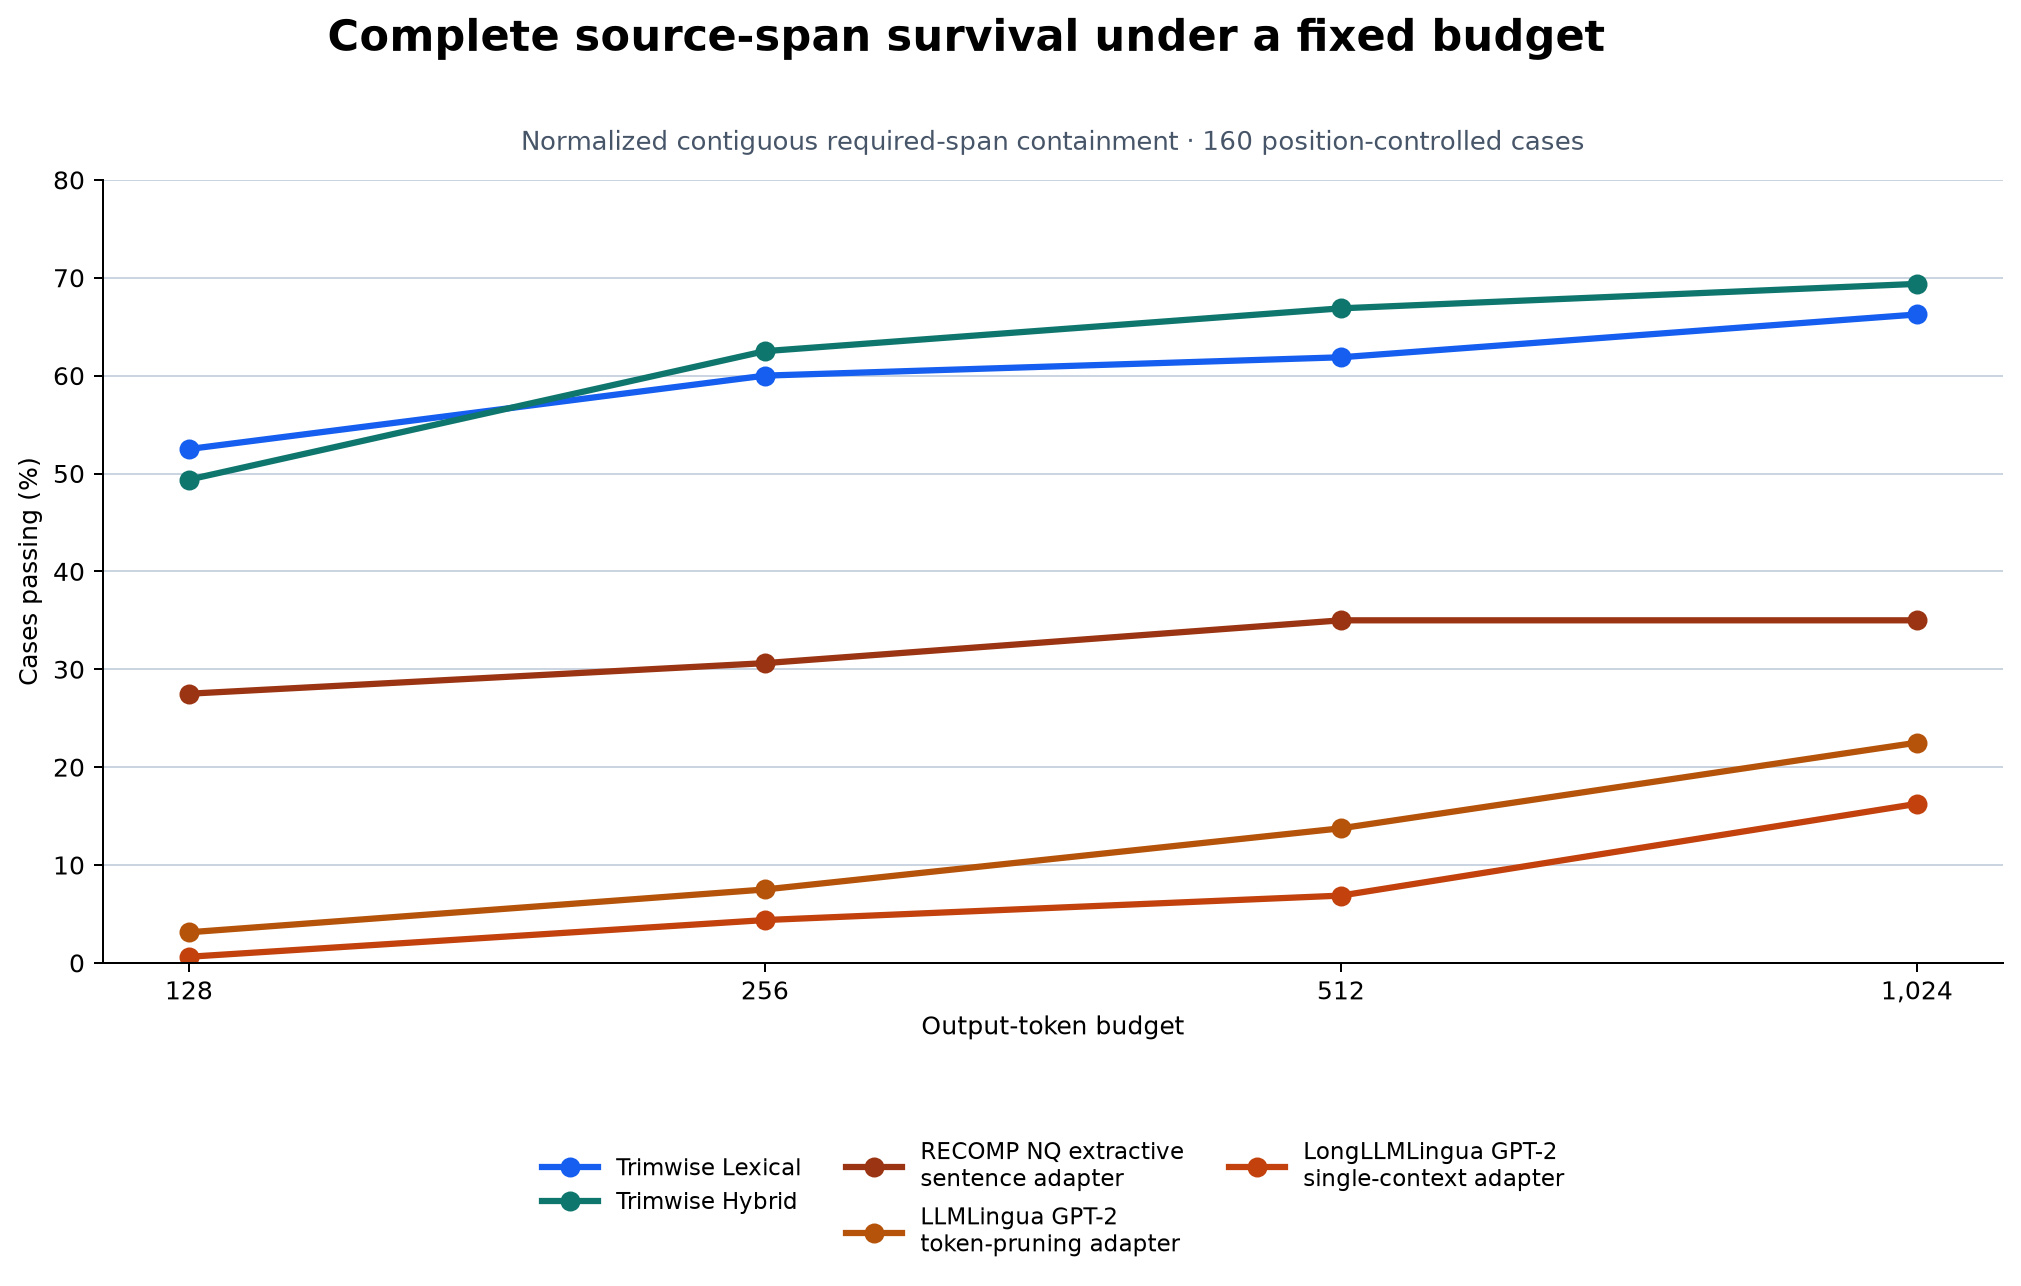
\includegraphics[keepaspectratio,alt={Normalized contiguous required-span containment by query-aware output-token budget.}]{../../../benchmark/reports/evidence-sensitivity-v1-2/normalized_contiguous_vs_budget.png}}
\caption{Normalized contiguous required-span containment by query-aware
output-token budget. The 160-case all-case rate is the primary v1.2 result;
the local ordered 80\% and 90\% sensitivity summaries are released alongside
the figure.}
\end{figure}

\begin{figure}
\centering
\pandocbounded{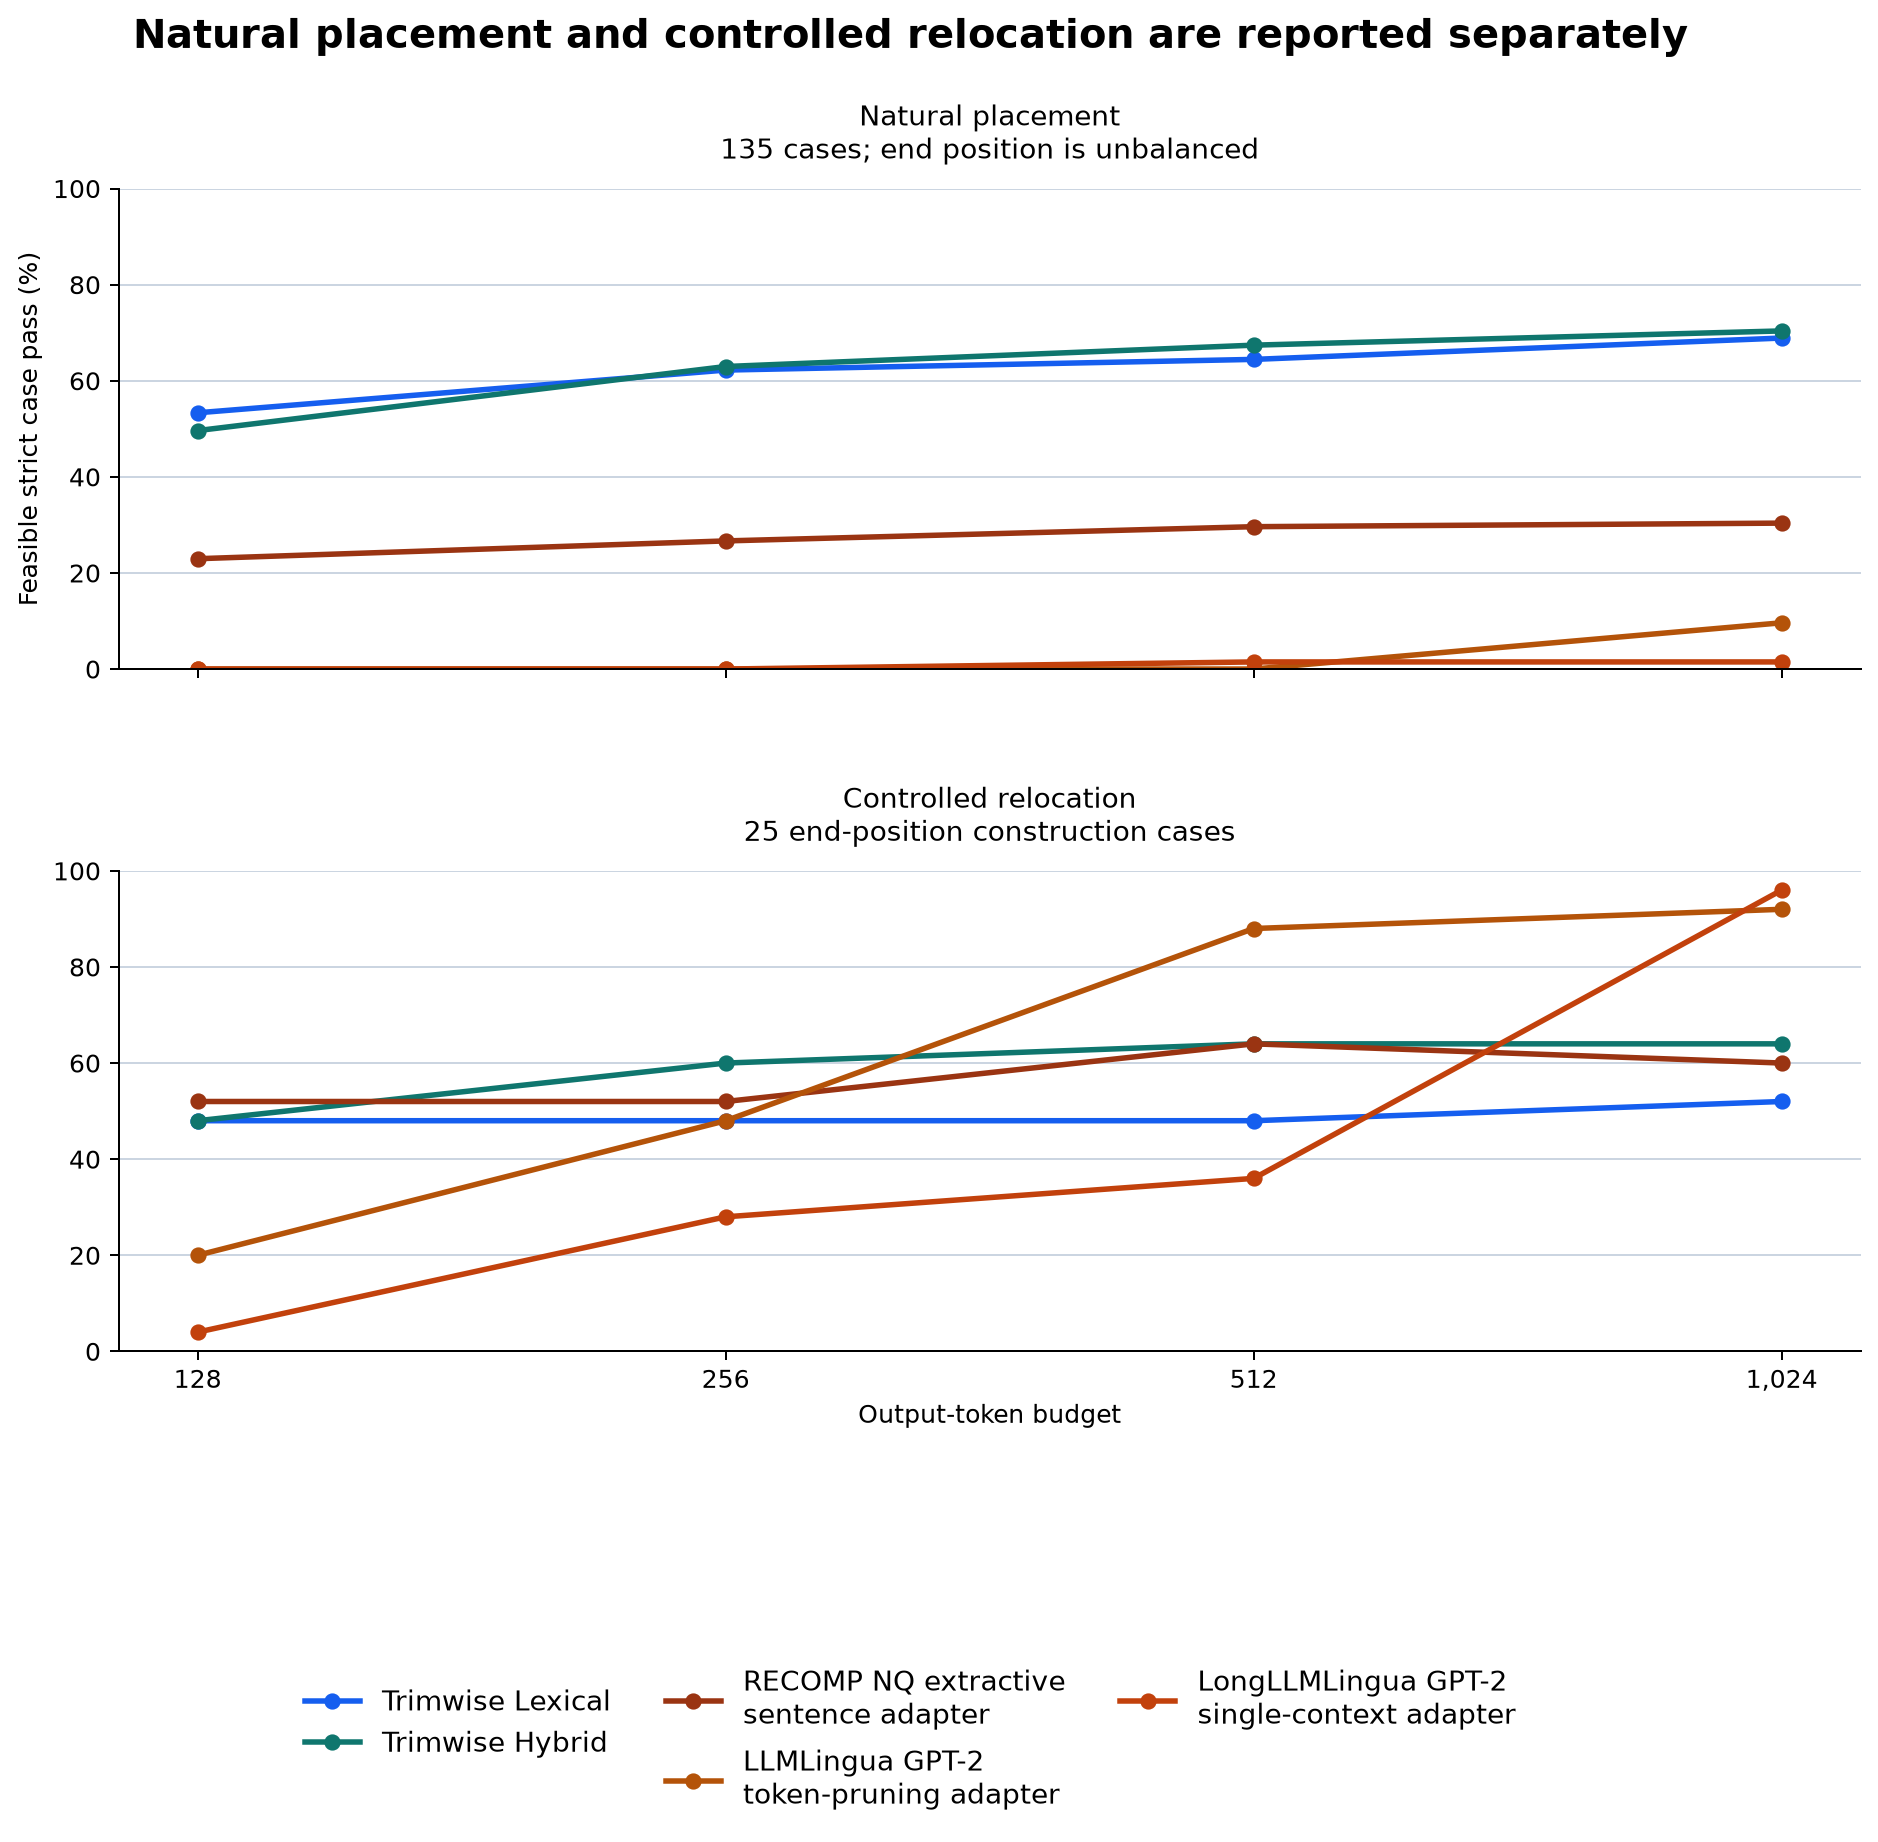
\includegraphics[keepaspectratio,alt={Strict source-span case pass shown separately for natural placement and controlled relocation cohorts.}]{../../../benchmark/reports/evidence-sensitivity-v1-2/natural_vs_relocated.png}}
\caption{Strict v1.2 cohort sensitivity. The top panel uses the 135 natural
placements and is unbalanced by position because it contains 15 natural end
cases. The bottom panel uses 25 controlled end relocations. It is a construction
diagnostic, not a causal estimate of naturally occurring end-evidence behavior.}
\label{fig:strict-cohort-sensitivity}
\end{figure}

Increasing the ceiling helps every evaluated adapter, but not to the same
extent. Hybrid rises from 49.4\% to 69.4\% normalized contiguous
containment between 128 and 1,024 tokens, while the RECOMP NQ extractive
sentence adapter rises from 27.5\% to 35.0\%. The LLMLingua GPT-2
token-pruning adapter rises from 3.1\% to 22.5\%, and the
LongLLMLingua GPT-2 single-context adapter rises from 0.6\% to 16.2\%.
Neither overtakes either Trimwise configuration on this suite.

The strict natural-only sensitivity preserves the same observed ordering
without claiming position balance. At 256 tokens, Hybrid passes 63.0\% of
the 135 natural cases and Lexical passes 62.2\%, compared with 26.7\% for
the RECOMP NQ extractive sentence adapter. At 1,024 tokens, the corresponding
rates are 70.4\%, 68.9\%, and 30.4\%. Excluding the ten cases drawn from
Trimwise's own documents leaves 150 rows: Hybrid passes 63.3\% at 256 tokens
and 67.3\% at 1,024 tokens, compared with 32.0\% and 36.7\% for RECOMP.
These checks use the same frozen compression strings; they do not create an
independent evaluation set.

The controlled-relocation cohort behaves differently and must remain
separate. At 256 tokens, Hybrid passes 60.0\% of the 25 relocated rows and
RECOMP passes 52.0\%, versus 63.0\% and 26.7\% on natural rows. At 1,024
tokens, the corresponding relocated rates are 64.0\% and 60.0\%, while
their natural rates are 70.4\% and 30.4\%. Relocation therefore changes more
than a global position label for some methods, plausibly through local context
and the composition of the remaining source. The combined 40-case end stratum
is useful for the balanced diagnostic, but not an estimate of naturally
occurring end-evidence performance.

The paired v1.2 bootstrap intervals show a positive Hybrid--RECOMP difference
under the primary metric at every budget: +21.9 percentage points (95\%
interval [+13.1, +31.2]) at 128 tokens, +31.9 [+22.5, +41.2] at 256,
+31.9 [+21.9, +41.9] at 512, and +34.4 [+25.0, +43.8] at 1,024. The full
paired table includes both Trimwise configurations and the two local ordered
sensitivities. These intervals describe resampling variation within this fixed,
author-annotated suite; they do not establish population-level superiority.

The additional budget is not always filled. Hybrid's median output is
126, 253, 253, and 263 tokens at the four ceilings; Lexical's is 126,
253, 269, and 271. In contrast, RECOMP's median output is 128, 255, 512,
and 1,023. This is expected from Trimwise's relevance-pool and selection
logic: its budget is a ceiling, not a requirement to append lower-ranked
evidence. Whether leaving capacity unused is desirable depends on a
downstream task; its source-level benefit here should not be read as
proof that a shorter excerpt always produces a better answer.

Strict v1.2 position-level results are also uneven. At 256 tokens, Hybrid
passes 77.5\% for beginning evidence, 65.0\% for middle evidence, 62.5\%
for end evidence, and 45.0\% for multiple-span evidence. Lexical records
72.5\%, 65.0\%, 57.5\%, and 45.0\% in the same order; RECOMP records
35.0\%, 40.0\%, 32.5\%, and 15.0\%. Multiple evidence remains the hardest
condition for both Trimwise configurations at all four budgets. Balancing
positions prevents early evidence from concealing that failure mode; it does
not make the strata equally difficult.

\subsection{Downstream Answer
Transfer}\label{downstream-answer-transfer}

Figure~\ref{fig:downstream-answer-match} reports the downstream diagnostic
directly. The dashed reference is the complete source under the same prompt
and evaluator, while each solid line receives a budgeted compressed context.
The source-evidence result transfers only partly to generated answers.
Across the 93 answerable cases, full context reaches 44.1\%, 45.2\%, and
45.2\% answer match for GPT-5.4 Nano, GPT-5.4 Mini, and GPT-5.6 Luna
respectively. Trimwise Hybrid reaches 46.2\% for Nano at 256 and 512
tokens, 46.2\% for Mini at 256 and 1,024 tokens, and 45.2\% for Luna at
256--1,024 tokens. Lexical reaches a similar range, including 47.3\% for
Nano at 1,024 tokens. The competing compressed contexts score
substantially lower under the same metric; for example, RECOMP ranges
from 8.6\% to 17.2\% for Nano and 7.5\% to 15.1\% for Mini across the
four budgets.

\begin{figure}
\centering
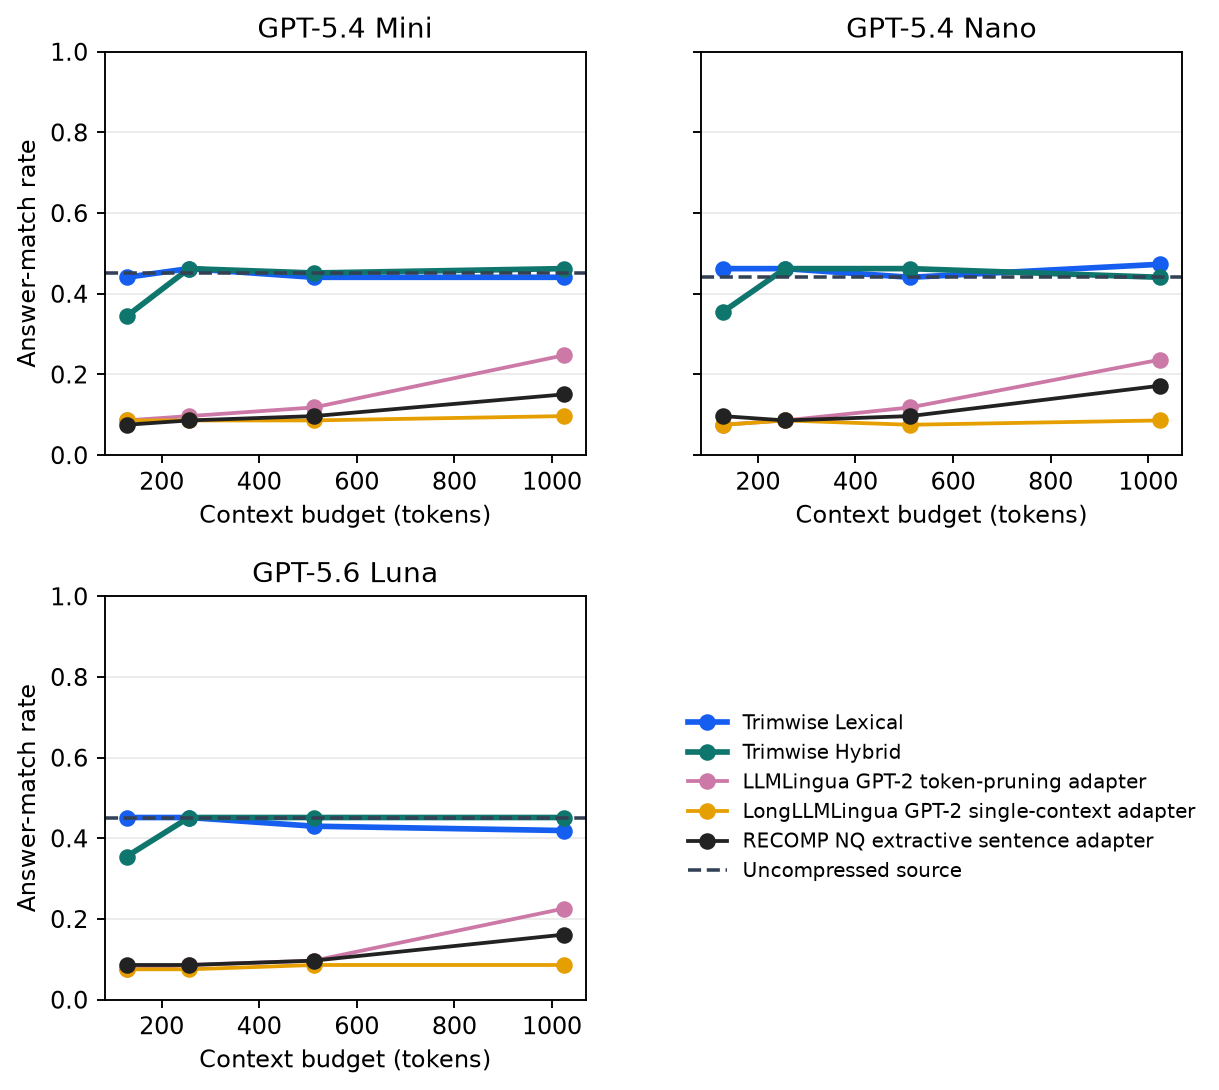
\includegraphics[width=\linewidth]{../../../benchmark/reports/query-aware/answer_pass.png}
\caption{Downstream answer-match rate on the 93 answerable cases. Solid
lines show compressed contexts at each token budget; the dashed line aggregates
one complete-source answer per case with the same prompt and evaluator. Answer
match is the automatic token-containment measure defined in Section~5.6;
each point uses one sampled completion. The complete-source line has no
compression budget and is a reference, not a guaranteed upper bound on
generated-answer quality.}
\label{fig:downstream-answer-match}
\end{figure}

The answer diagnostic is intentionally secondary to source-evidence
selection. Its automatic token-containment rule is permissive, each
context receives one nondeterministic generation, and public-source
knowledge may contribute to an answer. Within that diagnostic, Trimwise
excerpts remain near the complete-source reference at several budgets,
while the evaluated comparator outputs are lower. Repeated,
task-validated downstream evaluation is needed to assess generated-answer
quality more directly.

\subsection{Budget Compliance and
Runtime}\label{budget-compliance-and-runtime}

Every one of the 6,400 saved compression calls returned a successful
runner status. Under the shared counter, the LLMLingua GPT-2 token-pruning
adapter exceeded the ceiling in 196 of 640 query-aware calls (30.6\%), with
a maximum 139-token overflow, and the LongLLMLingua GPT-2 single-context
adapter did so in 357 calls (55.8\%), with a maximum 169-token overflow.
Both Trimwise methods and the RECOMP NQ extractive sentence adapter have zero
measured violations. Their mean utilization differs: 72.1\% for Lexical,
69.8\% for Hybrid, and 99.3\% for the RECOMP adapter.

On the recorded machine, warm median trim time is 6.4 ms for Lexical,
42.8 ms for Hybrid, 126.2 ms for the RECOMP adapter, 168.0 ms for the
LLMLingua adapter, and 340.7 ms for the LongLLMLingua adapter. Median
per-call CUDA peak allocated memory is 343 MB for the Trimwise paths,
472 MB for the RECOMP adapter, 1,475 MB for the LLMLingua adapter, and
1,193 MB for the LongLLMLingua adapter. These figures include the benchmark
adapters and their resident framework state, and p95 latency remains large
for the model-backed methods (156 ms, 1,442 ms, 1,161 ms, and 2,252 ms
respectively for Hybrid, the RECOMP adapter, the LLMLingua adapter, and the
LongLLMLingua adapter). They characterize the documented runtime
configuration; portable speed or memory estimates require reproduction on a
specified machine.

\section{Analysis}\label{analysis}

\subsection{Component Scope}\label{what-this-study-does-not-ablate}

This study compares complete deployed configurations. Lexical and Hybrid
differ in several operations: Hybrid requests semantic vectors, combines
normalized lexical and semantic scores, and can use dense similarity
during MMR. Their observed difference is consequently a
configuration-level effect, not an estimate of the individual
contributions of embeddings, score fusion, or dense diversity. The
comparisons with the RECOMP NQ extractive sentence adapter, the
LLMLingua GPT-2 token-pruning adapter, and the LongLLMLingua GPT-2
single-context adapter likewise combine differences in algorithm and
implementation stack.

The comparison still informs configuration choice on the evaluated
workload: Lexical is fastest and has the highest observed 128-token
normalized contiguous containment rate, while Hybrid is stronger at larger
ceilings. An ablation study would hold the source corpus and all other choices fixed
while varying segmentation granularity, lexical score, semantic score,
hybrid fusion, MMR, query-aware evidence cutoff, or source-order
reconstruction one at a time.

\subsection{Observed Failure Modes}\label{observed-failure-modes}

The results reveal four failure modes that matter more than the
aggregate curve. First, multiple required spans are difficult: under the
strict v1.2 metric, Hybrid reaches only 45.0\% case pass in that stratum
from 256 through 1,024 tokens. A single relevance-ranked fragment can be highly useful while
another necessary fragment is remote, weakly lexical, or excluded by the
evidence cutoff. Source-order reconstruction makes the selected pieces
readable; it does not solve the set-coverage problem.

Second, an underspecified query can rank related evidence above the
exact operational requirement. In \texttt{instruction-05-q1}, the query
is ``Evaluate an ordinary privacy deletion request.'' The required
source text is \texttt{RULE-5-A}, which specifies three required JSON
keys and prohibits Markdown. At the 1,024-token ceiling, Hybrid retains
a nearby but different threshold rule, \texttt{RULE-5-B}, about when
automatic approval is disallowed, while omitting \texttt{RULE-5-A}. The
saved result has no prohibited phrase and remains within budget, but
fails its sole required span. The failure is distinct from positional
truncation: the selector retrieves a semantically related policy
constraint that is insufficient for the task.

Third, the strict v1.2 case conjunction makes partial success visible as
failure. A method that retains three out of four required items receives
zero source-span-survival pass, even though its evidence F1 may be
nonzero. That is appropriate for tasks requiring every listed item, but it
means the metric should not be read as a smooth estimate of general
relevance. The evidence-F1 values and per-span coverage in the raw output
are necessary companions to the binary headline.

Fourth, generated answers can fail despite retained evidence or succeed
despite compression failure. The full-context reference's low
answer-match rate and possible public-data exposure make a downstream
answer an imperfect proxy for source use. This is why the paper treats
source-evidence selection as the primary measurement and generated
answers as a diagnostic. A future benchmark should include human review
or a stronger task-specific checker for a subset of cases before making
claims about reasoning quality.

\subsection{Configuration Trade-offs}\label{configuration-trade-offs}

Lexical has a
higher observed normalized contiguous containment rate than Hybrid at the
128-token ceiling and is about seven times faster in median warm trimming
time. If a query
shares distinctive terms with a short required span, BM25-style ranking
may be enough; a semantic backend adds cost without a guaranteed
benefit. At larger budgets, the RECOMP NQ extractive sentence adapter closes
part of the gap and uses nearly all available capacity. Applications whose task rewards broad
retained coverage rather than concise exact evidence may reasonably
choose that trade-off after validating it on their own documents.

\subsection{Qualitative Trace}\label{qualitative-trace}

The \texttt{instruction-05-q1} case illustrates the value of provenance
separate from the benchmark score. The required interval can be
identified in the original source as the exact
\texttt{RULE-5-A} span at character offsets 435--541. The saved Hybrid
output at 1,024 tokens contains the exact but different
\texttt{RULE-5-B} threshold text, plus background blocks and omission
markers. Retaining source identity and spans makes the omitted
output-schema rule inspectable; a compressed string alone leaves the
omission harder to diagnose. This trace is illustrative and complements
the quantitative results.

\section{Discussion}\label{discussion}

\subsection{Interpretation of Results}\label{what-the-results-establish}

Within this position-controlled benchmark, supplying a query materially
changes the context-selection problem. The two query-aware Trimwise
configurations retain required source evidence more often than the
evaluated query-aware comparators at all four ceilings and satisfy the
shared token counter more reliably. These findings concern selection
from one already-chosen source under the supplied annotations, adapter
configurations, and budgets.

The implementation contributes a separate output contract. Trimwise
composes exact source slices under its configured measurement rule,
preserves source order, and exposes original Python-string spans for
retained ranges. These properties let an application map a retained
fragment or an omission back to its own file, revision, and line
metadata.

\subsection{Operational Trade-offs}\label{operational-trade-offs}

Trimwise Lexical is the economical choice in the evaluated
configuration: it requires no managed embedding model and has a 6.4 ms
median warm trim time. Hybrid adds semantic-backend inference, increasing
the median to 42.8 ms, and is stronger at the larger budget ceilings in
this suite. These measurements depend on the embedding backend, cache,
CUDA configuration, and hardware.

Extractive fidelity is also a trade-off. Because Trimwise returns source
wording rather than a rewritten summary, it cannot compress several
dispersed facts into a new compact sentence. The benefit is recoverable
evidence and readable source order; the cost is that a tiny budget may
not fit all required fragments. Systems that permit an abstractive,
non-citable summary should evaluate that different design directly
rather than assuming an extractive selector is the right tool.

\subsection{Intended Operating Conditions}\label{appropriate-use-cases}

Trimwise is designed for applications that have already selected one
document or excerpt, have an informative task query, and need to reserve
a fixed portion of a larger prompt for exact source text. Typical
settings include optional repository excerpts while required
instructions remain outside the excerpt budget, policy or runbook
evidence for a focused question, and reviewable source passages whose
application-level identifiers and character spans can be converted to
citations.

\subsection{Settings Requiring Additional Safeguards}\label{inappropriate-use-cases}

The method is unsuitable as the sole mechanism when a task requires
synthesis across every qualification in a long document, when a query is
too vague to distinguish the needed rule from related rules, or when
meaning depends on omitted connectors, layout, or tables. Medical,
legal, financial, employment, and other high-impact decisions require
inspection of the authoritative source and explicit review for omitted
exceptions.

\subsection{Threats to Validity}\label{threats-to-validity}

The benchmark is partly author-constructed and uses source-evidence
annotations designed alongside the system being evaluated. Position
balancing reduces one visible bias but does not establish
representativeness across languages, genres, naturally occurring long
documents, or real agent workflows. Twenty-five end cases are controlled
relocations rather than natural end evidence. Public sources may be
present in downstream-model training data; synthetic sources do not
remove all forms of benchmark construction bias. The instruction-track
failure further shows that a query can be insufficiently specific for a
required operational rule.

Baseline behavior depends on adapter choices, internal tokenizers,
checkpoint identifiers, and hardware. The RECOMP NQ extractive sentence
adapter is built around a released checkpoint. The released runtime manifest
records the run's hardware and package state; reported latency also includes
the observed cache and process state. Finally, one
downstream API completion per context does not separate selector quality
from model sampling behavior. Independent reproduction on additional
task suites is needed to assess how these factors transfer.

\section{Conclusion}\label{conclusion}

Trimwise is an extractive context-selection system for selecting
source-backed text from one already-chosen document under a strict token,
word, or character ceiling. Its output contract preserves verbatim source
text and source order, returns original Python-string spans, and
distinguishes omission markers from source content.

On the 160-case position-controlled query-aware evaluation, Trimwise
Lexical and Hybrid achieved higher observed normalized contiguous
required-span containment than the evaluated LLMLingua GPT-2
token-pruning adapter, LongLLMLingua GPT-2 single-context adapter, and
RECOMP NQ extractive sentence adapter at 128, 256, 512, and 1,024 tokens.
The same ordering holds under local ordered 80\% and 90\% sensitivities.
The evaluation also exposes instruction-survival and multiple-span
failures.

These findings support query-aware, source-faithful selection for prompt
assembly from a known source under a hard budget. Priority next steps are
evaluation on independent task suites, including component ablations and
repeated downstream answer assessments.

\section{Limitations}\label{limitations}

Trimwise is extractive. It cannot synthesize a concise statement from
facts distributed across omitted regions, resolve contradictions, or
guarantee that selected text contains every material qualification.
Strict budget compliance and exact source spans therefore do not imply
task utility, truthfulness, safety, or contextual completeness. The
query-aware paths depend on the query's specificity, segmentation,
lexical overlap, and, for semantic or hybrid mode, the embedding model.
The instruction and multiple-evidence failures in this study are
concrete examples of those limits.

The evidence base is also limited. The 160-case dataset mixes public and
controlled synthetic documents, has author-designed source annotations,
and contains controlled end relocations. It does not establish results
for other languages, document types, private institutional corpora, or
production agent tasks. The API evaluator was sampled once per context,
uses a lightweight token-containment metric, and may know public-source
facts independently of the supplied context. No human answer assessment
or component ablation was performed.

The saved benchmark rows predate span metadata, although the 0.2.0
implementation comparison shows that adding spans does not change
selected text. The released runtime manifest records hardware, driver,
packages, model revisions, configuration, and result hashes after the
run. It supports traceability for this snapshot; it is not a portable
service-level performance claim.

\section{Ethical Considerations}\label{ethical-considerations}

Selection can create a misleading excerpt even when every retained
character is faithful to the source. Trimwise may omit qualifications,
warnings, dissenting evidence, scope conditions, or a later correction.
Users must not treat a selected passage as a complete or authoritative
representation of the document, especially in medical, legal, financial,
employment, safety, or other high-impact settings. Source spans make
auditing easier; they do not make an omission safe.

Applications are responsible for the privacy and access controls of the
sources and queries they provide. A caller-supplied embedding callback
may send source text to an external service, and a managed local model
may cache model artifacts; neither behavior is a substitute for
data-governance review. The benchmark's public-source material retains
its recorded license and attribution requirements. Controlled synthetic
cases are labeled as such, and their use should not imply that the
system has been validated on sensitive institutional material.

\section{Artifact Availability}\label{artifact-availability}

The immutable v1.1 research artifact is the annotated
\href{https://github.com/tenwritehq/trimwise/tree/paper-v1.1}{\texttt{paper-v1.1}
tag in the Trimwise repository}. It contains the original Trimwise
implementation; frozen source and 160-case position-controlled datasets;
source, method, and runtime manifests; raw compression and downstream-QA JSONL
rows; aggregate summaries and paired statistics; HTML reports and figures; and
the manuscript source. The parallel v1.2 scorer and its pre-aggregate protocol
freeze are in the annotated
\href{https://github.com/tenwritehq/trimwise/tree/paper-v1.2}{\texttt{paper-v1.2}
tag}; the original strict all-case summary, manifest, and protocol identify the
frozen 6,400 compression rows. This revision adds saved-output subgroup,
self-source-exclusion, and paired-bootstrap analyses under that unchanged v1.2
metric. Its complete manuscript, source, raw rows, derived CSVs, reports, and
PDF are released as the annotated
\href{https://github.com/tenwritehq/trimwise/tree/paper-v1.3}{\texttt{paper-v1.3}
tag}. The runtime manifest retains its historical \,\texttt{paper-v1} release
label because it records the original compression run; it is not the v1.2
scorer manifest. Reproduction commands are recorded in
\texttt{benchmark/README.md}; the manuscript build command is recorded in
\texttt{assets/paper/latex/README.md}.

\section{Acknowledgments}\label{acknowledgments}

The author thanks the maintainers and contributors of Python, NumPy, PyTorch,
Transformers, FastEmbed, Tiktoken, Hugging Face Hub, the OpenAI Python library
and Responses API, the LLMLingua implementation, and the released RECOMP
checkpoint. These tools and artifacts enabled implementation or evaluation;
their use does not imply endorsement. The corresponding research contributions
and model artifacts are cited where they inform the method or comparison.

\subsection{AI-Assisted Writing
Disclosure}\label{ai-assisted-writing-disclosure}

Generative AI tools assisted with manuscript organization and language
editing. The author designed the method and evaluation, inspected the
implementation and saved benchmark artifacts, verified the cited
literature, and remains responsible for the claims, results, and errors
in this manuscript.

\appendix

\section{Algorithm Specification}\label{algorithm-specification}

\subsection{Inputs, early exits, and ranking
text}\label{inputs-early-exits-and-ranking-text}

\texttt{trim(text,\ limit,\ unit,\ strategy,\ query,\ token\_counter)}
first validates its types, resolves \texttt{auto} to Lexical when
\texttt{query.strip()} is nonempty and to Structural otherwise, and
creates a measurement object for tokens, words, characters, or a caller
token counter. A zero limit returns the empty string. If the complete
input already fits, it returns that exact input without segmentation or
embedding work, with the sole span \texttt{{[}0,\ len(text))} for a
nonempty string.

Otherwise, the segmenter parses Markdown-aware blocks and uncovered raw
ranges into source-backed \texttt{Segment} values. Each value holds its
original half-open offsets, exact text, kind, section, and nearest
heading index. Only Structural mode expands a sole oversized plain-text
paragraph into complete sentences or source lines when possible.
Semantic ranking receives context-enriched passages containing a
repeated candidate and local section context; the selected text always
remains the original \texttt{Segment.text}, not the enriched ranking
passage.

\subsection{Selection pseudocode}\label{selection-pseudocode}

\begin{Shaded}
\begin{Highlighting}[]
\NormalTok{INPUT: source D, ordered segments U, ranking R, limit B, measurer m}
\NormalTok{OUTPUT: composed text T and original{-}input spans P}

\NormalTok{if strategy is STRUCTURAL:}
\NormalTok{    E \textless{}{-} all segment indexes}
\NormalTok{    try to add the first and last indexes together}
\NormalTok{    if both do not fit, try the structurally more relevant endpoint}
\NormalTok{    partition remaining indexes by section}
\NormalTok{    give each section an equal provisional share of remaining budget}
\NormalTok{    greedily add fitting candidates by live MMR within each section}
\NormalTok{else:}
\NormalTok{    E \textless{}{-} all non{-}heading indexes, or all indexes if there are no non{-}headings}
\NormalTok{    order E by primary score, then relevance, then source index}
\NormalTok{    find the greatest adjacent primary{-}score drop among the first ceil(0.9 * (|E|{-}1)) gaps}
\NormalTok{    retain candidates through that gap plus five later candidates, capped at |E|}

\NormalTok{while E is not empty:}
\NormalTok{    i \textless{}{-} highest live MMR candidate, ties to lower source index}
\NormalTok{    for query{-}aware selection, first try \{selected, heading(i), i\} when a heading exists}
\NormalTok{    otherwise try \{selected, i\}}
\NormalTok{    accept the trial only if complete composition measures \textless{}= B}
\NormalTok{    if the best trial fails, try remaining candidates in current MMR order}
\NormalTok{    stop when none of the remaining trials fits}

\NormalTok{if no complete candidate was accepted:}
\NormalTok{    use the progressively smaller exact{-}source fallback}

\NormalTok{return measured text and maximal source spans}
\end{Highlighting}
\end{Shaded}

At every accepted primary candidate, MMR updates the greatest observed
similarity for the remaining candidates. Structural and Lexical use
sparse TF--IDF similarity; Semantic and Hybrid use the embedding
similarity interface. A stable source-index tie break is part of the
ranking contract. The greedy procedure is not a global knapsack
optimizer.

\subsection{Composition, fallback, and
spans}\label{composition-fallback-and-spans}

Composition sorts selected indexes by original source position. It first
tests source fragments plus minimal plain separators. For a source gap
containing non-whitespace content, it attempts the configured omission
marker only if the marked variant still fits; otherwise it retains the
plain separator. It similarly attempts affordable leading and trailing
omission markers. The final result performs one more full measurement
and raises an internal error rather than return an output above the
limit.

When no complete structural candidate fits, fallback progressively
considers source-backed paragraph, sentence, and line fragments, then
uses the longest exact prefix that fits. CJK terminal punctuation is
recognized during sentence splitting. This means a tiny budget can end
within an unpunctuated line; no smaller complete source unit exists in
that case.

For retained segments in source order, Trimwise emits maximal spans.
Whitespace gaps are merged into the enclosing span when they are copied
from the original source; gaps containing omitted source content form a
span boundary. Added separators and omission markers never appear in a
span. Spans are Python-string half-open offsets and are ordered,
non-overlapping, and merged when adjacent.

\section{Benchmark Construction}\label{benchmark-construction}

The frozen source corpus has 250 cases over 150 documents and SHA-256
\texttt{7b752ea79f19369fa151aa27f8bcfb33abdc48d9a9da609b655640e931c7d428}.
Its manifest records 18 adversarial, 54 evidence-QA, 30 instruction, 24
procedure, 24 structured, and 100 real-source cases. The dataset
manifest records 150 \texttt{legacy\_verified} cases and 100
\texttt{assistant\_authored\_source\_span} cases; these labels describe
the available provenance metadata, not an independent annotation study.
Each public source document has a source URL, available revision,
license, and token count in \texttt{source\_manifest.csv}; controlled
synthetic documents are CC0-1.0.

For a case with exactly one required span, evidence position is the span
midpoint divided by context length: below one third is beginning, above
two thirds is end, and the remaining interval is middle. Cases with more
than one required span are classified as multiple. The builder takes 40
diverse natural cases each from beginning, middle, and multiple strata,
keeps all 15 natural end cases, and creates 25 end variants to reach 40.
A variant moves one unique required span unchanged to the end of the
same context, records its original offsets and parent case identifier,
and excludes that parent from the natural selection. Variant sources are
distinct documents and are allocated across tracks as 8 real-source, 5
evidence-QA, 4 instruction, 4 procedure, 2 structured, and 2 adversarial
cases.

The construction script checks unique case identifiers, exact
40/40/40/40 position balance, exact span slicing, variant source
uniqueness, single occurrence of moved evidence, unchanged evidence
text, and exact reconstructed relocation. The generated review manifest
lists every case and each controlled variant's original and new offsets.
This procedure establishes deterministic artifact integrity; it does not
prove that synthetic or relocated tasks are representative of naturally
occurring document work.

\section{Downstream Prompt and
Evaluator}\label{downstream-prompt-and-evaluator}

The Responses API receives exactly the following template, where
\texttt{protected\_prefix}, \texttt{context}, and
\texttt{protected\_suffix} are case fields. The compressor sees only
\texttt{context}; the prompt's prefix and suffix remain outside its
budget.

\begin{Shaded}
\begin{Highlighting}[]
\NormalTok{\{protected\_prefix\}}

\NormalTok{CONTEXT:}
\NormalTok{\{context\}}

\NormalTok{\{protected\_suffix\}}

\NormalTok{Return only the concise answer. Do not add a label, explanation, or citation.}
\end{Highlighting}
\end{Shaded}

When a case does not define a prefix, the default is
\texttt{Answer\ only\ from\ the\ supplied\ context.} When it does not
define a suffix, the fallback is \texttt{Question:\ \{query\}}. The
evaluator stores \texttt{response.output\_text.strip()} and scores only
that continuation. Calls use the model identifiers, 128-token output
ceiling, \texttt{reasoning.effort="none"},
\texttt{text.verbosity="low"}, API timeout, and shared concurrency
stated in Section 5.5. There is no retry policy for saved API failures,
no temperature parameter, no hidden judge model, and no manual parsing
correction.

\section{Historical v1.1 Diagnostics}\label{historical-v1-1-diagnostics}

\subsection{Historical v1.1 paired case-pass
differences}\label{paired-case-pass-differences}

Table 3 is generated by \texttt{scripts/paired\_stats.py} from saved
query-aware compression outputs under the historical bag-of-token scorer.
Each row uses all 160 paired cases; the difference is Trimwise Hybrid minus
the named adapter in percentage points. It reports percentile-bootstrap
intervals only and no significance test.

{\def\LTcaptype{none} % do not increment counter
\begin{longtable}[]{@{}
  >{\raggedleft\arraybackslash}p{(\linewidth - 8\tabcolsep) * \real{0.1300}}
  >{\raggedright\arraybackslash}p{(\linewidth - 8\tabcolsep) * \real{0.2200}}
  >{\raggedleft\arraybackslash}p{(\linewidth - 8\tabcolsep) * \real{0.1600}}
  >{\raggedright\arraybackslash}p{(\linewidth - 8\tabcolsep) * \real{0.1800}}
  >{\raggedleft\arraybackslash}p{(\linewidth - 8\tabcolsep) * \real{0.3100}}@{}}
\toprule\noalign{}
\begin{minipage}[b]{\linewidth}\raggedleft
Budget
\end{minipage} & \begin{minipage}[b]{\linewidth}\raggedright
Comparator
\end{minipage} & \begin{minipage}[b]{\linewidth}\raggedleft
Difference
\end{minipage} & \begin{minipage}[b]{\linewidth}\raggedright
95\% interval
\end{minipage} & \begin{minipage}[b]{\linewidth}\raggedleft
Hybrid-only / comparator-only passes
\end{minipage} \\
\midrule\noalign{}
\endhead
\bottomrule\noalign{}
\endlastfoot
128 & LLMLingua GPT-2 token-pruning adapter & +46.9 & {[}38.1, 55.6{]} & 79 / 4 \\
128 & LongLLM\allowbreak Lingua GPT-2 single-context adapter & +50.0 & {[}41.9, 58.1{]} & 81 / 1 \\
128 & RECOMP NQ extractive sentence adapter & +17.5 & {[}8.8, 26.3{]} & 43 / 15 \\
256 & LLMLingua GPT-2 token-pruning adapter & +55.6 & {[}46.3, 64.4{]} & 98 / 9 \\
256 & LongLLM\allowbreak Lingua GPT-2 single-context adapter & +58.8 & {[}50.0, 67.5{]} & 100 / 6 \\
256 & RECOMP NQ extractive sentence adapter & +25.6 & {[}16.3, 35.0{]} & 55 / 14 \\
512 & LLMLingua GPT-2 token-pruning adapter & +51.2 & {[}41.9, 60.6{]} & 91 / 9 \\
512 & LongLLM\allowbreak Lingua GPT-2 single-context adapter & +58.8 & {[}50.0, 66.9{]} & 99 / 5 \\
512 & RECOMP NQ extractive sentence adapter & +18.8 & {[}8.8, 28.1{]} & 49 / 19 \\
1,024 & LLMLingua GPT-2 token-pruning adapter & +30.0 & {[}20.0, 40.0{]} & 64 / 16 \\
1,024 & LongLLM\allowbreak Lingua GPT-2 single-context adapter & +46.2 & {[}36.3, 56.3{]} & 86 / 12 \\
1,024 & RECOMP NQ extractive sentence adapter & +13.8 & {[}5.6, 21.9{]} & 35 / 13 \\
\end{longtable}
}

\subsection{Source-only results}\label{source-only-results}

{\def\LTcaptype{none} % do not increment counter
\begin{longtable}[]{@{}lrrrrr@{}}
\toprule\noalign{}
Method & 128 & 256 & 512 & 1,024 & Budget violations \\
\midrule\noalign{}
\endhead
\bottomrule\noalign{}
\endlastfoot
Prefix & 19.4\% & 23.1\% & 25.6\% & 46.3\% & 0.0\% \\
Head--tail & 25.0\% & 33.1\% & 44.4\% & 47.5\% & 0.0\% \\
Trimwise Structural & 16.3\% & 18.1\% & 21.9\% & 29.4\% & 0.0\% \\
LLMLingua, no query & 3.8\% & 8.1\% & 15.6\% & 39.4\% & 30.6\% \\
LLMLingua-2 & 0.0\% & 0.0\% & 0.6\% & 4.4\% & 57.3\% \\
\end{longtable}
}

All values are historical v1.1 case-pass rates over the same 160 cases.
This table is not comparable to Table 1: the query-aware methods receive
the case query during selection, whereas these methods do not.
At 256 tokens, prefix truncation passes 90.0\% of beginning-evidence cases
but only 2.5\% of end cases and 0\% of middle or multiple-evidence cases.
Head--tail reaches 67.5\%, 0\%, 50.0\%, and 15.0\% across those four
positions; Trimwise Structural reaches 10.0\%, 0\%, 62.5\%, and 0\%.
These historical source-only values are retained as a diagnostic of
positional behavior, not as support for the strict query-aware claim.

\section{Qualitative Failure Trace}\label{qualitative-failure-trace}

The following trace is drawn from a saved benchmark row, not constructed
after the result:

{\def\LTcaptype{none} % do not increment counter
\begin{longtable}[]{@{}
  >{\raggedright\arraybackslash}p{(\linewidth - 2\tabcolsep) * \real{0.5000}}
  >{\raggedright\arraybackslash}p{(\linewidth - 2\tabcolsep) * \real{0.5000}}@{}}
\toprule\noalign{}
\begin{minipage}[b]{\linewidth}\raggedright
Field
\end{minipage} & \begin{minipage}[b]{\linewidth}\raggedright
Value
\end{minipage} \\
\midrule\noalign{}
\endhead
\bottomrule\noalign{}
\endlastfoot
Case & \texttt{instruction-05-q1} \\
Query & \texttt{Evaluate\ an\ ordinary\ privacy\ deletion\ request.} \\
Required source interval & 435--541 \\
Required evidence &
\texttt{RULE-5-A:\ Return\ exactly\ three\ JSON\ keys:\ decision,\ reason,\ and\ escalation\_required;\ do\ not\ emit\ Markdown.} \\
Method and budget & Trimwise Hybrid, 1,024 tokens \\
Retained competing rule &
\texttt{RULE-5-B:\ Never\ auto-approve\ a\ privacy\ deletion\ amount\ above\ 9000\ units\ unless\ exception\ code\ EX-05\ is\ present.} \\
Outcome & Required span miss; no prohibited phrase; within budget; case
pass = false \\
\end{longtable}
}

The trace illustrates lexical/semantic relatedness without task
sufficiency. The selected threshold rule is relevant to privacy
deletion, but it does not satisfy the required output-format condition.
If this had been a real policy source, source identity plus returned
offsets would let an application show exactly what was omitted and
recover a line citation from the original file. The synthetic case does
not establish how often this explanation will be available in production
documents.

\section{Reproduction Checklist}\label{reproduction-checklist}

\begin{itemize}
\tightlist
\item[$\boxtimes$]
  Dataset source URLs, revisions where available, and licenses are
  recorded.
\item[$\boxtimes$]
  Position-controlled construction and validation are scripted.
\item[$\boxtimes$]
  Raw compression outputs, QA outputs, aggregation, plotting, and paired
  analysis are present.
\item[$\boxtimes$]
  Evaluator model identifiers, prompt, output ceiling, and concurrency
  are recorded.
\item[$\boxtimes$]
  Package versions and a \texttt{uv} lock file are present.
\item[$\boxtimes$]
  Seeds and row-resume identities are recorded.
\item[$\boxtimes$]
  Comparator failures are retained rather than silently dropped.
\item[$\boxtimes$]
  Primary citations in this manuscript were checked against primary or
  official sources.
\item[$\boxtimes$]
  The original raw outputs are frozen in the public \texttt{paper-v1} Git
  snapshot; the v1.2 rescore and this report's derived results are released
  with \texttt{paper-v1.3} (Section~\ref{artifact-availability}).
\item[$\boxtimes$]
  \url{benchmark/data/manifests/runtime_manifest.json} preserves a local
  hardware, driver, package, model-artifact, configuration, and result-hash
  snapshot. The manifest is released with the \texttt{paper-v1} snapshot;
  it remains post-run evidence rather than a portable performance claim.
\item[$\boxtimes$]
  The local benchmark environment resolves the repository's Trimwise
  0.2.0 package.
\item[$\square$]
  Independent human annotation or evaluation validates the task labels
  and answer metric.
\item[$\square$]
  A component ablation study isolates segmentation, ranking, diversity,
  and composition choices.
\end{itemize}

\bibliography{../references}

\end{document}
